\documentclass[a4paper,10pt]{report}
\usepackage{booktabs}
\renewcommand{\arraystretch}{1.3}
%----------------------------------------------------------------------------------------
%	FONT
%----------------------------------------------------------------------------------------
\usepackage[utf8]{inputenc}
\usepackage[T1]{fontenc}

%\usepackage[scaled=0.8]{beramono} % beramono or luximono give very nice ttfamily fonts

%----------------------------------------------------------------------------------------
%	PAGE LAYOUT
%----------------------------------------------------------------------------------------
\usepackage[toc,page]{appendix}

\textwidth = 410pt

\usepackage{fancyhdr}
\pagestyle{fancy}


\fancyhf{}

%\renewcommand{\sectionmark}[1]{\markright{\thesection.\ #1}}

%\nouppercase{\rightmark}

\lhead{\bfseries \nouppercase{\leftmark}}
\rhead{\bfseries \nouppercase{\rightmark}}
\lfoot{}
\rfoot{\bfseries Page \thepage}

\headwidth=1.1\textwidth
\renewcommand{\headrulewidth}{1.5pt}
\renewcommand{\footrulewidth}{1.5pt}
\fancyhfoffset[L]{24pt}
\fancyhfoffset[R]{24pt}

\fancypagestyle{plain}{%
\fancyhf{} % clear all header and footer fields
\headwidth=1.1\textwidth
\renewcommand{\headrulewidth}{1.5pt}
\renewcommand{\footrulewidth}{1.5pt}
\lhead{\bfseries \nouppercase{\leftmark}}
\rhead{\bfseries \nouppercase{\rightmark}}
%\lhead{\leftmark}
%\rhead{\rightmark}
\lfoot{}
\rfoot{\bfseries Page \thepage}
%\rfoot{Page \thepage}
\headwidth=1.1\textwidth
\fancyhfoffset[L]{24pt}
\fancyhfoffset[R]{24pt}
}

\newcommand{\mysection}[2]{%
                         \sectionmark{#1}%
                         \section{#2}%
                         \sectionmark{#1}%
                       }

%%%%%%%%%
%\renewcommand{\chaptermark}[1]{\markboth{\uppercase{\thechapter.\ #1}}{}}
%\renewcommand{\sectionmark}[1]{\markright{\uppercase{\thesection.\ #1}}}
%\newcommand{\helv}{\fontfamily{phv}\fontseries{b}\fontsize{9}{11}\selectfont}
%\lhead[\helv \thepage]{\helv \rightmark}
%\rhead[\helv \leftmark]{\helv \thepage}
%\cfoot{}
%----------------------------------------------------------------------------------------
%	OTHER PACKAGES and COMMANDS
%----------------------------------------------------------------------------------------
\usepackage{graphicx}
\usepackage{epstopdf}


\usepackage{float}
%\usepackage{tikz}
%\usepackage{tikz-uml} 
\usepackage{amsmath}

\usepackage{pifont}
\usepackage{fourier}
\usepackage{dingbat}

\usepackage{hyperref}

\newcommand{\reffig}[1]{figure \ref{fig:#1}}

\newcommand{\myparagraph}[1]{\paragraph{#1}\mbox{}\\}
%----------------------------------------------------------------------------------------
%	CUSTON LISTING SETTINGS
%----------------------------------------------------------------------------------------
\usepackage{listings}
\usepackage{lstcustom}
\renewcommand{\lstfontfamily}{\ttfamily}
%----------------------------------------------------------------------------------------
%	COLORS
%----------------------------------------------------------------------------------------

\definecolor{Lightgray}{gray}{.80}
\definecolor{lightgrey}{rgb}{0.9,0.9,0.9}

%----------------------------------------------------------------------------------------
%	TITLE PAGE
%----------------------------------------------------------------------------------------

% Front page: logo?

\title{BornAgain. }
\author{}

\usepackage{eso-pic}
\newcommand\BackgroundPic{%
\put(0,0){%
\parbox[b][\paperheight]{\paperwidth}{%
\vfill
\centering
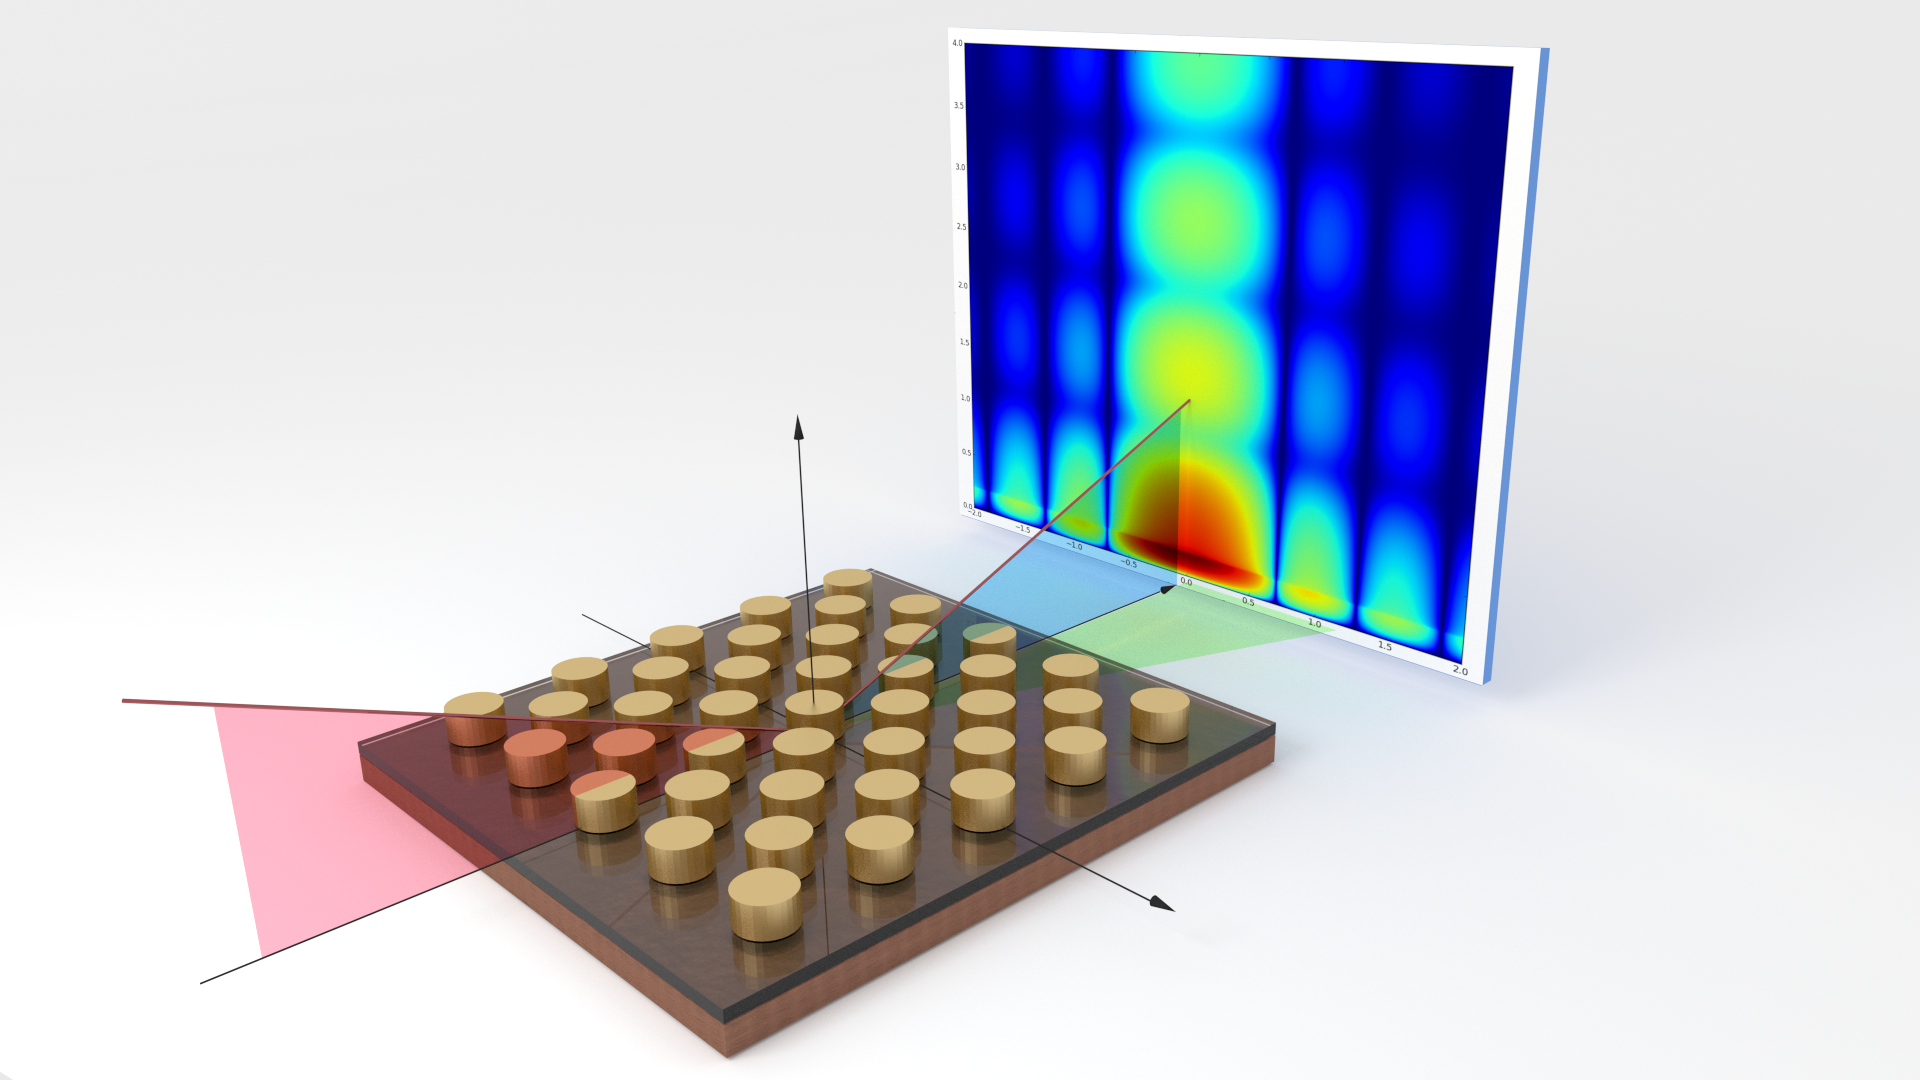
\includegraphics[width=\paperwidth,height=\paperheight,%
keepaspectratio]{results2_2.png}%
\vfill
}}}

%----------------------------------------------------------------------------------------
%	DOCUMENT
%----------------------------------------------------------------------------------------

\begin{document}

%\AddToShipoutPicture*{\BackgroundPic} % add background image to the
%first page
\maketitle


%\begin{abstract}
%This document describes the general architecture of the BornAgain project.
%\end{abstract}

\tableofcontents
\lstlistoflistings
\listoffigures
\listoftables

\newpage

BornAgain is a  software to simulate and fit neutron and X-ray
scattering at grazing incidence. It is a multi–platform open–source project that aims at supporting scientists in the analysis and fitting
of their GISAS data, both for synchrotron (GISAXS) and neutron (GISANS) facilities. The name of the software,
BornAgain, indicates the central role of the distorted-wave Born
approximation (DWBA) in the physical description of the
scattering process. The software provides a generic framework for modeling multilayer samples with smooth or
rough interfaces and with various types of embedded nanoparticles. In this way, it reproduces and enhances the
functionality of the present reference software, IsGISAXS by
R. Lazzari \cite{Lazzari:vi0158}, and lays a solid base for future
extensions in response to specific user needs. 

To meet the growing demand for GISAS simulation of more
complex structured materials, BornAgain has extended the IsGISAXS program’s functionality by removing the
restrictions on the number of layers and particles, by providing diffuse reflection from rough layer interfaces and
by adding particles with inner structure. \\


For details about the theory (DWBA,\ldots), please refer to IsGISAXS manual (\url{http://ln-www.insp.upmc.fr/axe4/Oxydes/IsGISAXS/figures/doc/manual.html}).\\


\colorbox{Lightgray}{\parbox{0.95\linewidth}
{
\noindent \underline{Icons used in this manual:}
\begin{itemize}
\item[] \smallpencil: this sign highlights further references.
%\item[] {\huge\ding{45}} - \smallpencil \textbf{\smallpencil}: this sign highlights further references.
\item[] {\huge\danger}: this sign highlights essential points.
\end{itemize}
}
}



%%%%%%%%%%%%%%%%%%%%%%%%%%%%%%%%%%%%%%%%%%%%%%%%%%%%%%%%%%%%%%%%%%%%%%%%%%%%%%%%
%%
%%   BornAgain User Manual
%%
%%   homepage:   http://www.bornagainproject.org
%%
%%   copyright:  Forschungszentrum Jülich GmbH 2015
%%
%%   license:    Creative Commons CC-BY-SA
%%   
%%   authors:    Scientific Computing Group at MLZ Garching
%%               C. Durniak, M. Ganeva, G. Pospelov, W. Van Herck, J. Wuttke
%%
%%%%%%%%%%%%%%%%%%%%%%%%%%%%%%%%%%%%%%%%%%%%%%%%%%%%%%%%%%%%%%%%%%%%%%%%%%%%%%%%


\cleardoublepage
\mychapter{0}{Introduction}

\BornAgain\
%\marginpar{scope}%
is a free and open-source software package
to simulate and fit small-angle
scattering at grazing incidence (GISAS)
with X-rays (GISAXS) or neutrons (GISANS).
It provides a generic framework
for modeling multilayer samples with smooth or
rough interfaces and with various types of embedded nanoparticles.
%\marginpar{name}%
The name, \BornAgain,
alludes to the central role of the distorted-wave Born
approximation (DWBA) in the physical description of the
scattering process.
\index{Distorted-wave Born approximation}

\BornAgain\
%\marginpar{extends \IsGISAXS}
almost completely reproduces the functionality
of the widely used program \IsGISAXS\
\index{IsGISAXS@\IsGISAXS}
\index{Lazzari, R\'emi}
by R\'emi Lazzari \cite{Laz02,Laz08}.
\BornAgain\ goes beyond \IsGISAXS\ by
supporting an unrestricted number of layers and particles, 
diffuse reflection from rough layer interfaces,
particles with inner structures, neutron polarization and magnetic scattering.
Adhering to a strict object-oriented design,
\BornAgain\ provides a solid base for future extensions
in response to specific user needs.

\BornAgain\
%\marginpar{platforms}%
\index{Platform|see {Operating system}}%
\index{Operating system}%
is operating system independent.
We actively support
Linux,
\index{Linux}%
MacOS
\index{MacOS}%
and  Microsoft Windows.
\index{Windows|see {Microsoft Windows}}%
\index{Microsoft Windows}%
%\marginpar{licence}%
It is a free and open source software under
the GNU General Public License (GPL, version 3 or higher).
This documentation is released under the Creative Commons license CC-BY-SA.
When \BornAgain\ is used in preparing scientific papers,
please cite software and manual as follows:
\index{Citation}%
%\marginpar{citation}%
\begin{quote}
C.~Durniak, M.~Ganeva, G.~Pospelov, W.~Van Herck, J.~Wuttke (2015),\newline
BornAgain --- Software for simulating and fitting
X-ray and neutron small-angle scattering at grazing incidence,
version \UserManualVersionNumber,\newline
\url{http://www.bornagainproject.org}
\end{quote}

This User Manual is complementary to the online documentation
at \url{http://www.bornagainproject.org}.
It does not duplicate information that is more conveniently read online.
Therefore, Sect.~\ref{sec:online} just contains a few pointers to the web site.
The remainder of this User Manual mostly contains background
on the sample models and on the scattering theory implemented in \BornAgain,
and some documentation of the corresponding \Python\ functions.
%Sect.~\ref{sec:Simulation} describes
%the general methodology of a simulation with \BornAgain,
%and gives detailed usage examples.
%Sect.~\ref{sec:ScatteringCrosssection} explains
%which sample structures are supported in \BornAgain,
%and which physical approximations are used.
%Fitting is explained in Sect.~\ref{sec:Fitting}.
%More theoretical background is given in Appendix~\ref{app:theory}.
%Implemented particle formfactors are specified in Appendix~\ref{app:ff}.

\Warn{\indent Software and documentation are work in progress.
We cannot guarantee that they are accurate and correct.
Anyway, it is entirely in the responsibility of users
to ensure that their data interpretation is physically meaningful.
If in doubt, please contact us.}

\index{Bug reports}
We are grateful for all kind of feedback:
criticism, praise, bug reports, feature requests or contributed modules.
If questions go beyond normal user support,
we will be glad to discuss a scientific collaboration.

%\newpage
\section{Installation} \SecLabel{Installation}

This section describes how to build and install \BornAgain\ libraries from the source.
At the moment we support building on x86/x86\_64 Linux and Mac OS X operating systems.
Support for Windows systems is planned in next releases.
%In the later releases we are planing to include support for Windows systems and provide
%binary distributions for major Windows/Mac/Linux.
There are three major steps to building \BornAgain\ :
\begin{enumerate}[1.]
\item Acquire required third-party libraries.
\item Get \BornAgain\ source code.
\item Use \Code{cmake} to build and install software.
\end{enumerate}
The remainder of this section explains each step in detail.

\subsection{Third-party software.}
To successfully build \BornAgain\ a number of prerequisite packages must be installed.

\begin{itemize}
\item compilers: clang  versions $\geq 3.1$ or GCC versions $\geq 4.2$
\item cmake ($\geq 2.8$)
\item boost library ($\geq 1.48$)
\item GNU scientific library ($\geq 1.15$)
\item fftw3 library ($\geq 3.3$)
\item python ($\geq 2.7$), python-devel, python-numpy-devel
\end{itemize}
\vspace*{2mm}

Other packages are optional
\begin{itemize}
\item ROOT framework (adds several additional fitting algorithms to \BornAgain)
\item python-matplotlib (allows to run usage examples with graphics)
%\item Eigen3 library ($\geq 3.1.0$)
\end{itemize}

All required packages can be easily installed on most Linux distributions using the system's package
manager. Below we give a few examples for several selected operation systems. Please note,
that other distributions (Fedora, Mint, etc) may have different commands for invoking the package manager and slightly different names of packages (like ``boost'' instead of ``libboost'' etc). Besides that, the installation should be very similar.
\vspace*{3mm}

% ---------------
%  OpenSuse 12.3
% ---------------
\noindent
{\large\bf OpenSuse 12.3} \newline
Adding ``scientific'' repository 
\begin{lstlisting}[language=shell, style=commandline]
sudo zypper ar http://download.opensuse.org/repositories/science/openSUSE_12.3 science
\end{lstlisting}

\noindent
Installing required packages
\begin{lstlisting}[language=shell, style=commandline]
sudo zypper install git-core cmake gsl-devel boost-devel fftw3-devel python-devel python-numpy-devel
\end{lstlisting}

\noindent
Installing optional packages
\begin{lstlisting}[language=shell, style=commandline]
sudo zypper install libroot-* root-plugin-* root-system-* root-ttf libeigen3-devel python-matplotlib
\end{lstlisting}
\vspace*{3mm}


% ---------------
%  Ubuntu 13.04
% ---------------
\noindent
{\large\bf Ubuntu 13.04} \newline
Installing required packages
\begin{lstlisting}[language=shell, style=commandline]
sudo apt-get install git cmake libgsl0-dev libboost-all-dev libfftw3-dev python-dev python-numpy
\end{lstlisting}

\noindent
Installing optional packages
\begin{lstlisting}[language=shell, style=commandline]
sudo apt-get install libroot-* root-plugin-* root-system-* ttf-root-installer libeigen3-dev python-matplotlib python-matplotlib-tk
\end{lstlisting}
\vspace*{3mm}


% ---------------
%  MacOS 10.8
% ---------------
\noindent
\noindent
{\large\bf Mac OS X 10.8} \newline
To simplify the installation of third party open-source software on a Mac OS X system we recommend the use of \Code{MacPorts} package manager. 
The easiest way to install MacPorts is by downloading the \Code{dmg} 
from \url{www.macports.org/install.php} and running the system's installer.
After the installation new command ``\Code{port}'' will be available in terminal window of your Mac. \

\noindent
Installing required packages
\begin{lstlisting}[language=shell, style=commandline]
sudo port -v selfupdate
sudo port install git-core cmake
sudo port install fftw-3 gsl
sudo port install boost -no_single-no_static+python27 


\end{lstlisting}

\noindent
Installing optional packages
\begin{lstlisting}[language=shell, style=commandline]
sudo port install py27-matplotlib py27-numpy py27-scipy
sudo port install root +fftw3+python27
sudo port install eigen3
\end{lstlisting}




\subsection{Getting source code}
\BornAgain\ source can be downloaded at \url{http://apps.jcns.fz-juelich.de/BornAgain}
and unpacked with
\begin{lstlisting}[language=shell, style=commandline]
tar xfz bornagain-<version>.tgz
\end{lstlisting}

\noindent
Alternatively one can obtain \BornAgain\ source from our public Git repository.
\begin{lstlisting}[language=bash, style=commandline]
git clone git://apps.jcns.fz-juelich.de/BornAgain.git 
\end{lstlisting}
\vspace*{3mm}


\noindent
{\bf\large More about Git} \\
Our Git repository holds two main branches called ``master'' and ``develop''. We consider ``master''
branch to be the main branch where the source code of HEAD always reflects latest stable release. \Code{git clone} command shown above
\begin{enumerate}[1.]
\item gives you a source code snapshot corresponding to the latest stable release,
\item automatically sets up your local master branch to track our remote master branch, 
so you will be able to fetch changes from the remote branch at any time using ``git pull'' command.
\end{enumerate}

Master branch is updating approximately once per month.
% that reflects our release cycle.
The second branch, ``develop'' branch, is a snapshot of the current development.
This is where any automatic nightly builds are built from. The develop branch is
always expected to work, so to get the most recent features one can switch source code to it by
\begin{lstlisting}[language=bash, style=commandline]
cd BornAgain
git checkout develop
git pull
\end{lstlisting}
\vspace*{3mm}



\subsection{Building and installing the code}

\BornAgain\ should be build using \Code{CMake} cross platform build system. 
Having third-party libraries installed on the system and \BornAgain\ source code acquired as was explained in
previous sections, type build commands
\begin{lstlisting}[language=bash, style=commandline]
mkdir <build_dir>
cd <build_dir>
cmake <source_dir> -DCMAKE_INSTALL_PREFIX=<install_dir>
make
\end{lstlisting}
\vspace*{3mm}

Here \Code{<source\_dir>} is the name of directory, where \BornAgain\ source code has been
copied, \Code{<install\_dir>} is the directory, where user wants  the package
to be installed, and \Code{<build\_dir>} is the directory where building will occur.

\MakeRemark{About \Code{CMake}}{
\\Having dedicated directory \Code{<build\_dir>} for build process
is recommended by \Code{CMake}. That allows several builds with different compilers/options from the same source and keeps source directory clean from build remnants. \\
}


Compilation process invoked by the command ``make'' lasts about 10 min for an average laptop
of 2012 edition. On multi-core machines the compilation time  can be decreased by invoking command
``make'' with the parameter ``make -j[N]'', where N is the number of cores.

Running functional tests is an optional but recommended step. Command ``make check''
will compile several additional tests and run them one by one. Every test contains
the simulation of a typical GISAS geometry and the comparison on numerical level of simulation results with reference files. Having 100\% tests passed ensures that your local installation
is correct.
\begin{lstlisting}[language=bash, style=commandline]
make check
...
100% tests passed, 0 tests failed out of 26
Total Test time (real) = 89.19 sec
[100%] Build target check
\end{lstlisting}
\vspace*{3mm}


The last command ``make install'' copies compiled libraries and some usage examples
into  the installation directory.
\begin{lstlisting}[language=bash, style=commandline]
make install
\end{lstlisting}


\subsubsection{Troubleshooting}

In the case of complex system setup, with variety of libraries of different versions 
scattered across multiple places (\Code{/opt/local}, \Code{/usr} etc.),
you may want to help \Code{CMake} to find libraries in proper place. 
In example below
two system variables are defined to force \Code{CMake} to prefer libraries
found in \Code{/opt/local} to other places.
\begin{lstlisting}[language=bash, style=commandline]
export CMAKE_LIBRARY_PATH=/opt/local/lib:$CMAKE_LIBRARY_PATH
export CMAKE_INCLUDE_PATH=/opt/local/include:$CMAKE_INCLUDE_PATH
\end{lstlisting}


If compilation fails for some reason, please submit your bug report including compilation errors
at \url{http://apps.jcns.fz-juelich.de/redmine/projects/bornagain/issues}



\subsection{What is next?}

In your installation directory you will find
\begin{lstlisting}[language=bash, style=commandline]
./include - header files for compilation of your C++ program
./lib - libraries to import into python or link with your C++ program
./Examples - directory with examples
\end{lstlisting}

Run your first example and enjoy first BornAgain simulation plot.
\begin{lstlisting}[language=bash, style=commandline]
cd <install_dir>/Examples/python/ex001_CylindersAndPrisms
python CylindersAndPrisms.py
\end{lstlisting}








%\documentclass[a4paper,10pt]{article}
\usepackage[utf8]{inputenc}
\usepackage[T1]{fontenc}
\usepackage{float}
\usepackage{tikz}
\usepackage{tikz-uml} 
\usepackage{amsmath}

\newcommand{\reffig}[1]{figure \ref{fig:#1}}

%opening
\title{}
\author{}

\begin{document}

%\maketitle

\begin{abstract}
This document describes the general architecture of the BornAgain project.
\end{abstract}

\section{Data classes for simulations and fits}
This section will give an overview of the classes that are used to describe all the data needed to perform a single simulation. The prime elements of this data are formed by the sample, the experimental conditions (beam and detector parameters) and simulation parameters.

These classes constitute the main interface to the software's users, since they will mostly be interacting with the program by creating samples and running simulations with specific parameters. Since it is not the intent to explain internals of classes in this document, the text and figures will only mention the most important methods and fields of the classes discussed. Furthermore, getters and setters of private member fields will not be indicated, although these do belong to the public interface. For more detailed information about the project's classes, their methods and fields, the reader is referred to the source code documentation. REF?

\subsection{The Experiment object}
The Experiment class holds all references to data objects that are needed to perform a simulation. These consist of a sample description, possibly implemented by a builder object, detector and beam parameters and finally, a simulation parameter class that defines the different approximations that can be used during a simulation. Besides getters and setters for these fields, the class also contains a runSimulation() method that will generate an ISimulation object that will perform the actual computations. The class diagram for Experiment is shown in \reffig{exp}.

\vspace{8mm}
\begin{figure}[H]
%the makebox macro ensures centering of the resulting figure
\makebox[\textwidth][c]{
\begin{tikzpicture}
\begin{umlpackage}{Simulation Data}
\umlclass{Experiment}{
  -- mp\_sample : ISample* \\
  -- mp\_sample\_builder : ISampleBuilder* \\
  -- m\_detector : Detector \\
  -- m\_beam : Beam \\
  -- m\_intensity\_map : OutputData<double> \\
  -- m\_sim\_params : SimulationParameters
}{
  \umlvirt{+ clone() : Experiment*} \\
  \umlvirt{+ runSimulation() : void} \\
  \umlvirt{+ normalize() : void}
}
\umlemptyclass[x=7, y=0]{ISample}
\umlemptyclass[x=7, y=-2]{Detector}
\umlemptyclass[x=7, y=-4]{Beam}
\umlemptyclass[x=7, y=-6]{SimulationParameters}
\umlemptyclass[y=-4]{GISASExperiment}
\umluniassoc[geometry=|-, anchor1=0]{Experiment}{ISample}
\umluniassoc[geometry=|-, anchor1=0]{Experiment}{Detector}
\umluniassoc[geometry=|-, anchor1=0]{Experiment}{Beam}
\umluniassoc[geometry=|-, anchor1=0]{Experiment}{SimulationParameters}
\umlinherit[geometry=--]{GISASExperiment}{Experiment}

\umlnote[y=-6.5, width=6cm]{GISASExperiment}{
  The ``runSimulation()'' method retrieves an ISimulation object
  from the topmost ISample object and calls its ``run()'' method 
  to perform the actual computations.
}
\end{umlpackage}
\end{tikzpicture}
} %end makebox
\caption{The Experiment class as a container for sample, beam, detector and simulation parameters.}
\label{fig:exp}
\end{figure}

\subsection{The ISample class hi\"erarchy}

Samples are described by a hi\"erarchy tree of objects which all adhere to the ISample interface. The composite pattern is used to achieve a common interface for all objects in the sample tree. The sample description is maximally decoupled from all computational classes, with the exception of the ``createDWBASimulation()'' method. This method will create a new object of type ``DWBASimulation'' that is capable of calculating the scattering contributions originating from the sample in question. The coupling is however not very tight, since the ISample subclasses only need to know about which class to instantiate and return.

This interface and two of its subclasses are sketched in \reffig{isample}.

\vspace{8mm}

\begin{figure}[H]
\makebox[\textwidth][c]{
\begin{tikzpicture}
\begin{umlpackage}{Sample description} 
% Code from official documentation goes here...
\umlinterface{ISample}{
}{
  \umlvirt{+ clone() : ISample*} \\
  \umlvirt{+ createDWBASimulation() : DWBASimulation*}
}
\umlclass[y=-4]{MultiLayer}{
  -- m\_layers : std::vector<Layer *> \\
  -- m\_interfaces : std::vector<LayerInterface *>
}{
  + getNumberOfLayers() : size\_t \\
  + getNumberOfInterfaces() : size\_t \\
  + addLayer(const Layer \&layer) : void
}
\umlclass[x=8,y=-4]{Layer}{
  -- mp\_material : IMaterial* \\
  -- m\_thickness : double
}{
  + getThickness() : double \\
  + setThickness(double thickness) : void
}
\umlinherit[geometry=-|]{MultiLayer}{ISample}
\umlinherit[geometry=|-]{Layer}{ISample}
\umluniassoc[geometry=--, mult2=n]{MultiLayer}{Layer}
\end{umlpackage}
\end{tikzpicture}
}
\caption{The ISample interface}
\label{fig:isample}
\end{figure}

\end{document}

%%%%%%%%%%%%%%%%%%%%%%%%%%%%%%%%%%%%%%%%%%%%%%%%%%%%%%%%%%%%%%%%%%%%%%%%%%%%%%%%%
%%
%%   BornAgain:  simulate and fit scattering at grazing incidence
%%
%%   homepage:   http://www.bornagainproject.org
%%
%%   copyright:  Forschungszentrum Jülich GmbH 2015
%%               Software licence does not cover this documentation
%%               For documentation licence, contact the authors
%%   
%%   authors:    Scientific Computing Group at MLZ Garching
%%               C. Durniak, M. Ganeva, G. Pospelov, W. Van Herck, J. Wuttke
%%
%%%%%%%%%%%%%%%%%%%%%%%%%%%%%%%%%%%%%%%%%%%%%%%%%%%%%%%%%%%%%%%%%%%%%%%%%%%%%%%%


\newpage
\chapter{Fitting} \SecLabel{Fitting}

In addition to the simulation of grazing incidence
X-ray and neutron scattering by
multilayered samples, \BornAgain\ also offers the option to
fit the numerical model to reference data by modifying a selection of
sample parameters from the numerical model.  This aspect
of the software is discussed in the current chapter.

%\SecRef{FittingGentleIntroducion} gives a short introduction to the
%basic concepts of data fitting. Users familiar with fitting can
%directly proceed to \SecRef{FittingImplementation}, which details the
%implementation of fittings in 
%\BornAgain\ . 
\SecRef{FittingImplementation} details the
implementation of fittings in \BornAgain\ . 
\Python\ fitting examples with detailed
explanations of every fitting step are given in \SecRef{FittingExamples}. Advanced fitting techniques, including fine tuning of minimization
algorithms, simultaneous fits of different data sets, parameters
correlation, are covered in
\SecRef{FittingAdvanced}. \SecRef{FittingRightAnswers} contains some practical advice, which might
help the user to get right answers from \BornAgain\ fitting.

%%%%%%%%%%%%%%%%%%%%%%%%%%%%%%%%%%%%%%%%%%%%%%%%%%%%%%%%%%%%%%%%%%%%%%%%%%%%%%%%
%
%%%%%%%%%%%%%%%%%%%%%%%%%%%%%%%%%%%%%%%%%%%%%%%%%%%%%%%%%%%%%%%%%%%%%%%%%%%%%%%
\section{Gentle introduction to the data fitting.} \SecLabel{FittingGentleIntroducion}

The aim of this section is to briefly introduce the basic concept of
data fitting, its key terminology and difficulties which might arise in scattering data fit.
Users wanting to find out more about minimization (also called
maximization or optimization methods depending on the formulations and objectives) 
or looking for more rigorous discussion than provided in this manual
are referred to \cite{Antoniou2007, mntutorial}

\subsection{Toy scattering experiment.}

Fig.~\ref{fig:toyfit_data},left shows scattering intensity map in arbitrary units  
as a function of (x,y) of the detector ``measured'' in toy scattering experiment.

\begin{figure}[!p]
  \centering
    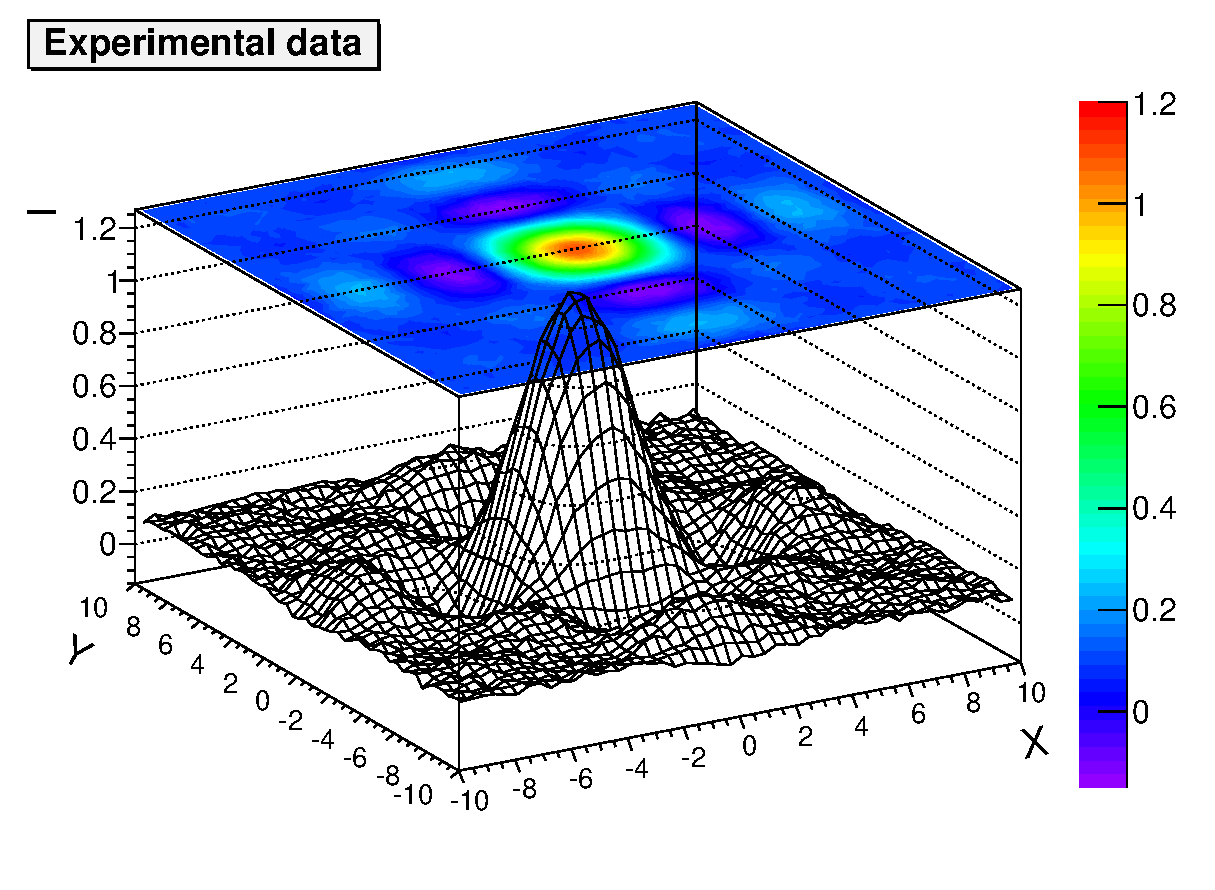
\includegraphics[width=0.49\textwidth]{Figures/toyfit_expdata.eps}
    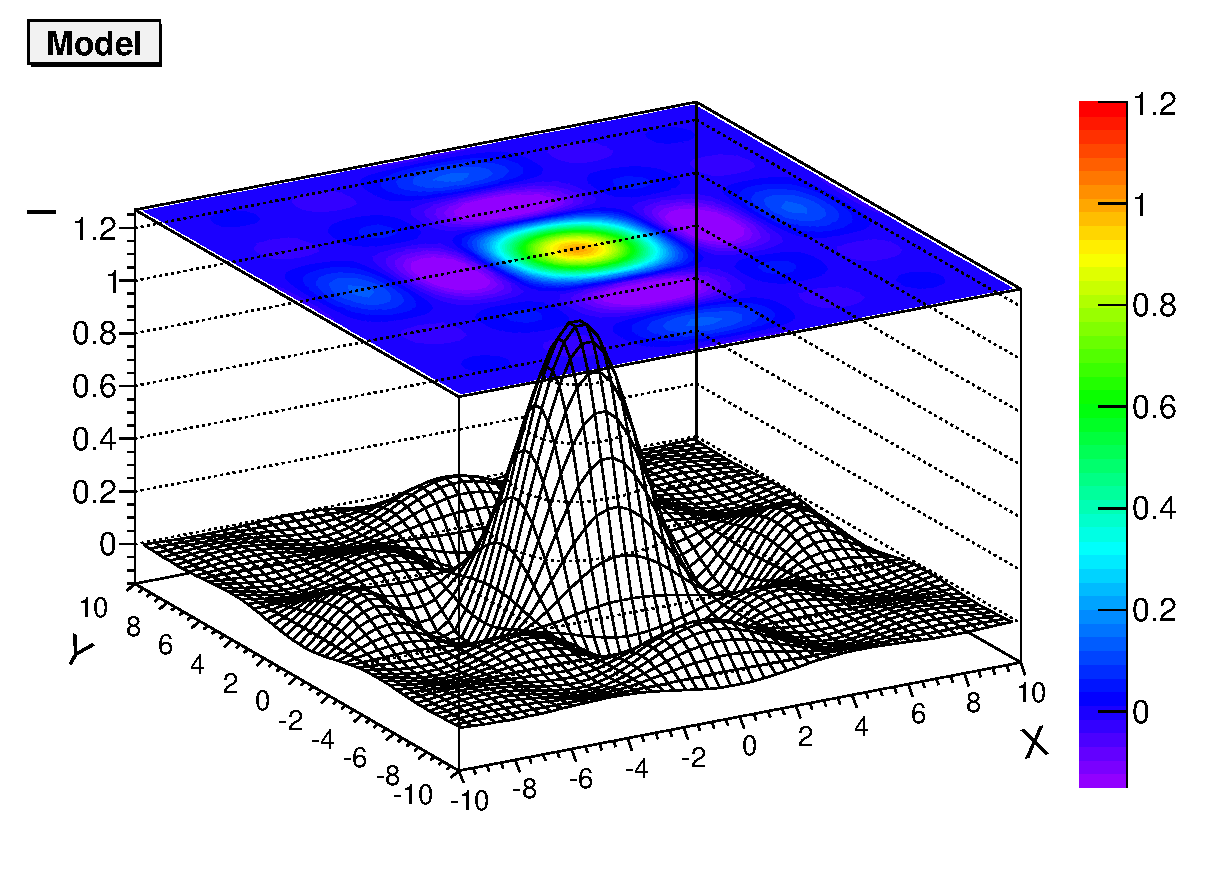
\includegraphics[width=0.49\textwidth]{Figures/toyfit_simdata.eps}
  \caption{Intensity as a function of (x,y) detector coordinates  obtained from 
  toy experiment (left) and from the toy simulation (right).   }
  \label{fig:toyfit_data}
  \vspace*{4mm}
    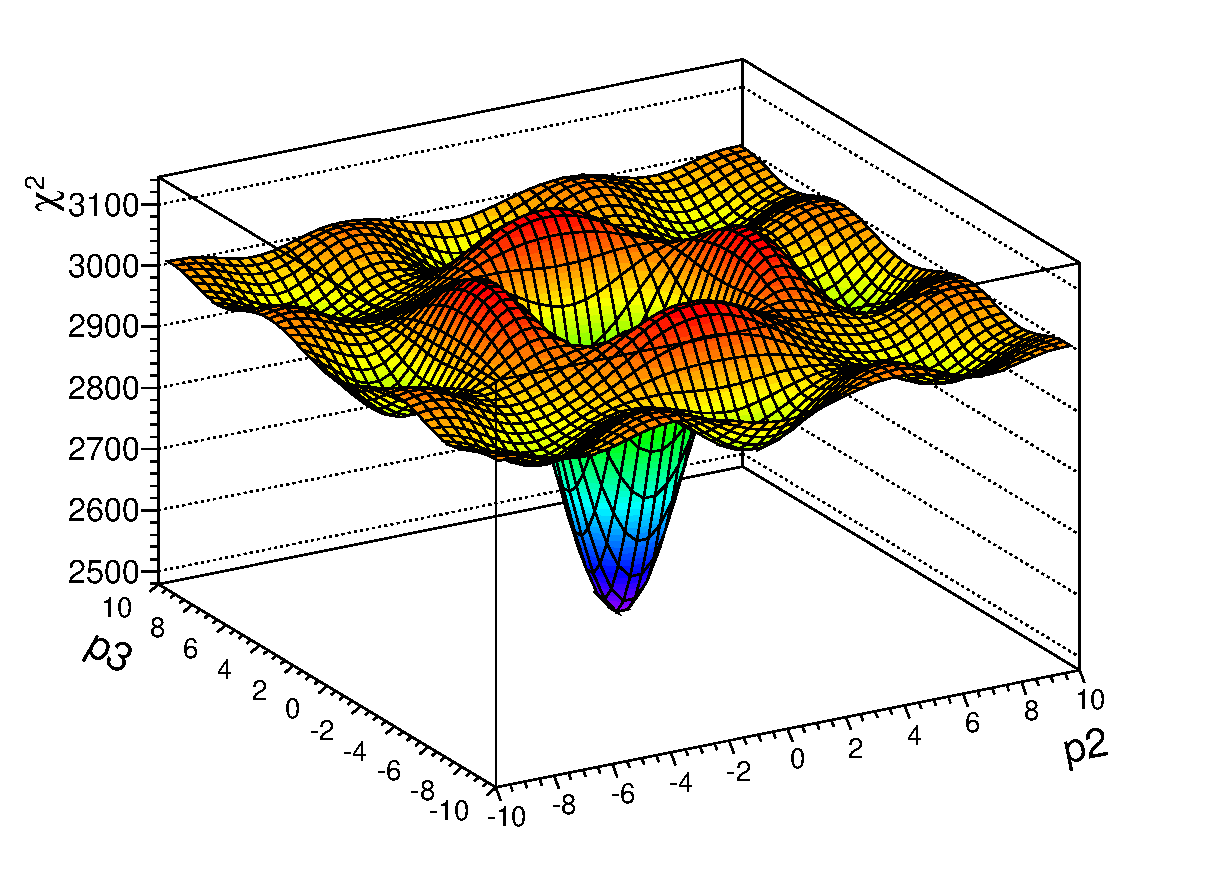
\includegraphics[width=0.49\textwidth]{Figures/toyfit_chi2_p23.eps}
    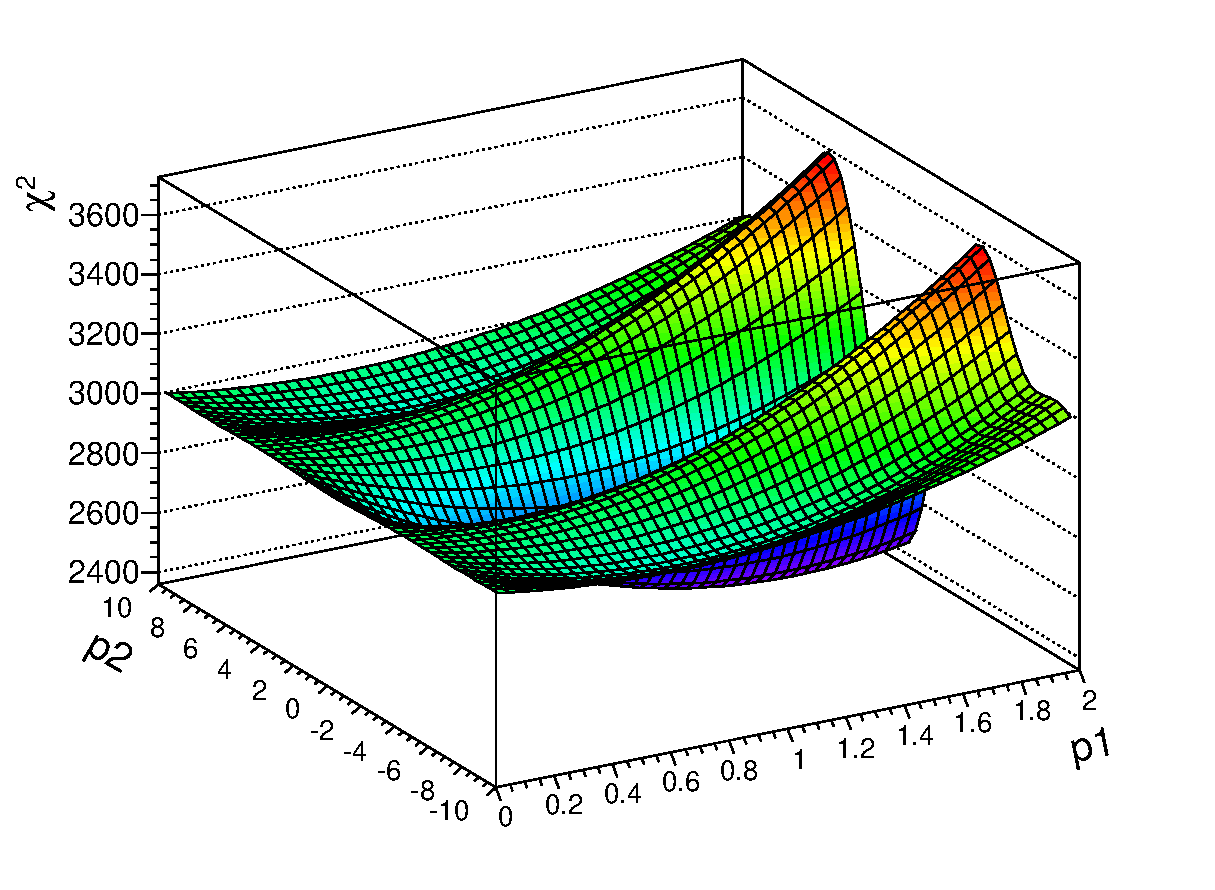
\includegraphics[width=0.49\textwidth]{Figures/toyfit_chi2_p12.eps}
  \caption{$\chi^{2}$ value calculated between experimental and simulated data
  as a function of $p_2,p_3$ parameters (left) or $p_1,p_2$ 
  parameters (right) used in the model.   }
  \label{fig:toyfit_chi2}
\end{figure}


Scattering picture presented reminds some of GISAS patterns, nevertheless it is
generated using simple function
$$I(x,y) = G(0.1,~0.01) + \frac{sin(x)}{x} \cdot \frac{sin(y)}{y}$$
Here $G(0.1, 0.01)$ is a random variable distributed according to the Gaussian distribution
with mean 0.1 and $\sigma=0.01$.
Constant $0.1$ symbolize our experimental background and constant $0.01$ is referred
to the detector noise. The rest of the formula represents our signal.

Lets define our model, namely specific mathematical function, to which we will fit our toy experimental data. By making an educated guess we assume that scattering intensity observed
in the experiment should be described with the help of $sinc$ function as follows
$$ f(x,y) = p_0 + p_1 \cdot  sinc(x - p_2) \cdot sinc(y - p_3) $$
The model has four parameters: $p_0$ describing background, $p_{1}$ describing signal strength
and $p_2,p_3$ responsible for the peak position.
Fig.~\ref{fig:toyfit_data},right shows the intensity as a function (x,y) calculated according
our model using fixed parameter set $p_0=0,p_1=1,p_2=0,p_3=0$. 

Two distributions look pretty much the same, however to find exact values of parameters which describe experimental data in the best way, one have to
\begin{itemize}
\item elaborate criteria for the difference between an actual data and its model
\item employ minimization procedure which will minimize that difference
\end{itemize}


\subsection{Objectives}

The goal is to obtain the best fit of an observed distribution
to a prediction by modifying a set of parameters from the
prediction. This problem can be one or multi-dimensional and also linear or
nonlinear. The quantity to minimize is often referred to as the
\textit{objective function}, whose expression depends on the
particular method, like the maximum likelihood, the $\chi^2$
minimization or the expected prediction error function. 

\begin{comment}
\subsubsection*{Maximum of likelihood.}
This is a popular method for parameters' estimations because the maximum likelihood estimators are approximately
unbiased and efficient for large data samples, under quite general
conditions.
We assume a sample  $\mathbf{x}=\{x_{1},x_{2},...,x_{n}\}$ of n independent and identically distributed
observations coming from probability density function $f(\mathbf{x}; \mathbf{p})$.
We assume $f(\mathbf{x}; \mathbf{p})$
to be known except for the parameters $\mathbf{p}=\{p_1,p_2,...,p_3\}$
The method of maximum likelihood takes the estimators to be
those values of $\mathbf{p}$ that maximize the likelihood function $\mathcal{L}$ as
$\mathcal{L}(\mathbf{\alpha})=\prod_{i=1}^N f(x_i;\mathbf{p})$.
Since it is easier to deal with a sum, we usually minimize
$-\text{ln}(\mathcal{L})$.
\end{comment}


\subsubsection*{$\chi^2$ or least squares minimization}
A dataset consist of $n$ data pairs $(\mathbf{x_{i}}, a_{i}), i=1,N$ where 
$\mathbf{x_{i}}$ is an independent variable and $a_{i}$ is dependent variable, whose
value is found in the measurement $i$. The number $N$ denotes the total
number of measurements. 

In the case of intensity map measured in our toy experiment 
and presented in Fig~\ref{fig:toyfit_data}, a variable $a_{i}$ denotes measured intensity, a variable $\mathbf{x_{i}}$ is a vector and correspond to the 
$(x_{i}, y_{i})$ coordinates of pixels in our detector while number $N$  corresponds 
to total number of detector pixels.

The model function has the form
$f(\mathbf{x_{i}},\mathbf{p})$
where adjustable parameters are held in the vector $\mathbf{p}$.
The least squared method finds the optimum of model function which 
fit the data in the best way by searching for the minimum of the sum of squared
residuals
$$ \chi^{2}(\mathbf{p}) = \sum_{i=1}^{N}r_{i}^{2}$$
where residual is defined as the difference between measured value and the value predicted by the model.
$$r = a_{i} - f(\mathbf{x_{i}},\mathbf{p})$$

In the case of normally distributed variables with the $\sigma^2$ variance
the quantity to minimize becomes
$$ \chi^{2}(\mathbf{p}) =
\frac{1}{d}
\sum_{i=1}^{N}  
\frac{ (a_{i} - f(\mathbf{x_{i}},\mathbf{p}))^2}{\sigma^2}   $$
where $d=N-k$ is number of degree of freedom ($k$ number of free fit parameters).


\subsubsection*{Minimization algorithms}
There are a large number of minimization algorithms providing a solution to the problem
of minimizing the objective function over the space of parameters of the function.
The minimization starts from initial guess for the parameters provided by the user,
and then evolves iteratively under control of minimization algorithm. The procedural
modifications on the parameters, the objective function, as well as convergence
criterion depend on the method implemented.
Details of particular implementation is beyond the scope of this manual and
 interested reader is encouraged to look at outside resources.



\subsubsection*{Local minima trap}




\subsection{Terminology.}

\noindent
{\bf Reference data} \\
Normally just experimental data or might be also simulated data
spoiled with the noise for purpose of testing of minimization algorithms.
\vspace*{1mm}

\noindent
{\bf Objective function} \\
Subject of minimization procedure.
\vspace*{1mm}

\noindent
{\bf Minimization} \\
Finding a best available values (i.e. local minimum) of some objective function. 
\vspace*{1mm}

\noindent
{\bf Number of degrees of freedom} \\
Number of data points - number of parameters in the fit.
\vspace*{1mm}

\noindent
{\bf Minimizer} \\
An algorithm which minimize objective function. 



%%%%%%%%%%%%%%%%%%%%%%%%%%%%%%%%%%%%%%%%%%%%%%%%%%%%%%%%%%%%%%%%%%%%%%%%%%%%%%%
%
%%%%%%%%%%%%%%%%%%%%%%%%%%%%%%%%%%%%%%%%%%%%%%%%%%%%%%%%%%%%%%%%%%%%%%%%%%%%%%%
\section{Implementation in BornAgain} \SecLabel{FittingImplementation}

Fitting in  \BornAgain\ deals with estimating the optimum parameters
in the numerical model by minimizing the difference between
numerical and reference data.
%using $\chi^2$  or maximum likelihood methods. 
The features include 

\begin{itemize}
\item a variety of multidimensional minimization algorithms and strategies.
\item the choice over possible fitting parameters, their properties and correlations.
\item the full control on objective function calculations, including applications of different normalizations and assignments of different masks and weights to different areas of reference data.
\item the possibility to fit simultaneously an arbitrary number of data sets.
\end{itemize}

Figure ~\ref{fig:minimization_workflow} shows general work flow of a typical fitting procedure.
\begin{figure}[htbp]
\centering
  \resizebox{0.99\textwidth}{!}{%
    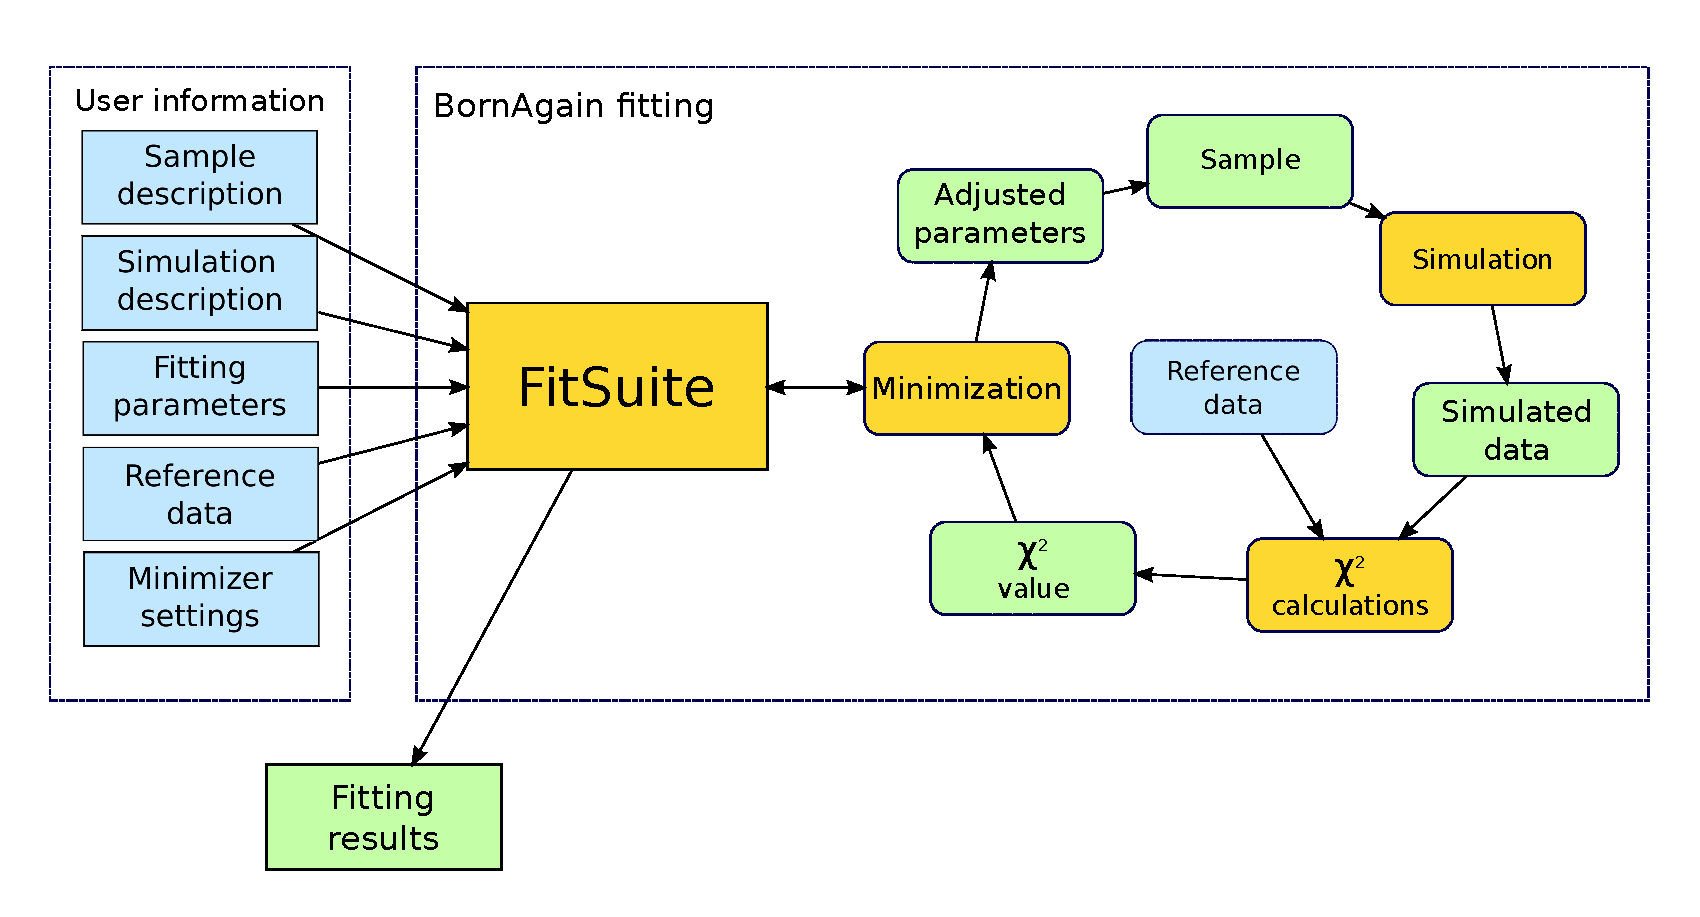
\includegraphics{Figures/minimization_workflow.eps}}
\caption{
Fitting work flow.
}
\label{fig:minimization_workflow}
\end{figure}

Before running the fitting the user is required to prepare some  data and to
configure the fitting kernel of \BornAgain\ . The required stages are

\begin{itemize}
\item Preparing the sample and the simulation description (multilayer, beam, detector parameters).
\item Choosing the fitting parameters.
\item Loading the reference data.
\item Defining the minimization settings.
\end{itemize}

The class \Code{FitSuite} contains the main functionalities to be used for the fit
and serves as the main interface between the user and the fitting work flow. 
The later involves iterations during which

\begin{itemize}
\item The minimizer makes an assumption about the optimal sample parameters.
\item These parameters are propagated to the sample.
\item The simulation is performed for the given state of the sample.
\item The simulated data (intensities) are propagated to the $\chi^2$ module.
\item The later calculates $\chi^2$ using the simulated and reference data.
\item The value of $\chi^2$ is propagated to the minimizer, which makes new assumptions about optimal sample parameters.
\end{itemize}

The iteration process is going on under the control of the selected minimization
algorithm, without any intervention from the
user. It stops 
\begin{itemize}
\item when the maximum number of iteration steps has been exceeded,
\item when the function's minimum has been reached within the tolerance window,
\item if the minimizer could not improve the values of the parameters. 
\end{itemize}

After the control is returned, fitting results can be retrieved.
They consist in the best $\chi^2$ value found, the corresponding
optimal sample parameters and the intensity map simulated with this set of parameters.

Details of \Code{FitSuite} class implementation and description
of each interface are given in \SecRef{FitSuiteClass}. The following parts of this section will detail each of
the main stages necessary to run a fitting procedure.


%%%%%%%%%%%%%%%%%%%%%%%%%%%%%%%%%%%%%%%%%%%%%%%%%%%%%%%%%%%%%%%%%%%%%%%%%%%%%%%
%
%%%%%%%%%%%%%%%%%%%%%%%%%%%%%%%%%%%%%%%%%%%%%%%%%%%%%%%%%%%%%%%%%%%%%%%%%%%%%%%
\subsection{Preparing the sample and the simulation description}

This step is similar for any simulation using \BornAgain\ (see \SecRef{Simulation}). It consists in first characterizing  the geometry of the system: the particles 
(shapes, sizes, refractive
indices), the different layers (thickness,
order, refractive index, a possible roughness of the interface), the
interference between the particles and the way they are distributed in
the layers (buried particles or particles sitting on top of a
layer). 
Then we specify the parameters of the input beam and of the
output detector.


%%%%%%%%%%%%%%%%%%%%%%%%%%%%%%%%%%%%%%%%%%%%%%%%%%%%%%%%%%%%%%%%%%%%%%%%%%%%%%%
%
%%%%%%%%%%%%%%%%%%%%%%%%%%%%%%%%%%%%%%%%%%%%%%%%%%%%%%%%%%%%%%%%%%%%%%%%%%%%%%%
\subsection{Choice of parameters to be fitted}
In principle, every parameter used in the construction of the sample
can be used as a fitting parameter. For example, the particles'
heights, radii or the layer's roughness or thickness could be selected
using the 
parameter pool mechanism. 
This mechanism is explained in detail in
\SecRef{WorkingWithSampleParameters} and it is therefore recommended
to read it before proceeding any further.

The user specifies selected sample parameters as fit parameters using \Code{FitSuite}
and its \Code{addFitParameter} method
\begin{lstlisting}[language=shell, style=commandline]
fit_suite = FitSuite()
fit_suite.addFitParameter(<name>, <initial value>, <step>, <limits>)
\end{lstlisting}
where \Code{<name>} corresponds to the parameter name in the sample's parameter pool.
By using wildcards in the parameter name, a group of sample parameters, corresponding to the given
pattern, can be associated with a single fitting parameter and 
fitted simultaneously to get a common optimal value (see \SecRef{WorkingWithSampleParameters}).

The second parameter \Code <initial value> correspond to the initial value of
the fitting parameter, while the third one
is responsible to the initial iteration steps size.
The last parameter \Code{<AttLimits>} corresponds to
the boundaries imposed on parameter value. It can be
\begin{itemize}
\item \Code{limitless()} by default, 
\item \Code{fixed()}, 
\item \Code{lowerLimited(<min\_value>)}, 
\item \Code{upperLimited(<max\_value>)}, 
\item \Code{limited(<min\_value>, <max\_value>)}.
\end{itemize}
where \Code{<min\_value>} and \Code{<max\_value>} are
double values corresponding to the lower and higher boundary, respectively.


%%%%%%%%%%%%%%%%%%%%%%%%%%%%%%%%%%%%%%%%%%%%%%%%%%%%%%%%%%%%%%%%%%%%%%%%%%%%%%%
%
%%%%%%%%%%%%%%%%%%%%%%%%%%%%%%%%%%%%%%%%%%%%%%%%%%%%%%%%%%%%%%%%%%%%%%%%%%%%%%%
\subsection{Associating reference and simulated data}

The minimization procedure deals with a pair of reference data (normally
associated with experimental data) and the theoretical model (presented by the sample and the simulation descriptions).

We assume that the experimental data are a two-dimensional intensity 
matrix as function of the output scattering
angles $\alpha_f$ and $\phi_f$ (see Fig.~\ref{fig:multil3d}).
The user is required to provide the data in the form of an ASCII file
containing an axes
binning description and the intensity data itself. 
\vspace*{2mm}

\ImportantPoint{Remark:}{
We recognize the importance of supporting the most common data formats. We are going to provide
this feature in the following releases and welcome users' requests on this subject.
}
\vspace*{1mm}

To associate the simulation and the reference data to the fitting engine, method \newline
\Code{addSimulationAndRealData} has to be used as shown
\begin{lstlisting}[language=python, style=eclipseboxed,numbers=none]
fit_suite = FitSuite()
fit_suite.addSimulationAndRealData(<simulation>, <reference>, <chi2_module>)
\end{lstlisting}

Here \Code{<simulation>} corresponds to a \BornAgain\ simulation object
with the  sample, beam and detector fully defined, \Code{<reference>}
corresponds to the experimental data object obtained from the ASCII file and \Code{<chi2\_module>} is an optional parameter for advanced 
control of $\chi2$ calculations.

It is possible to call this given method more than once to submit more than one pair of
\Code{<simulation>, <reference>} to the fitting procedure.
In this way, simultaneous fits of
some combined data sets are performed.

By using the third \Code{<chi2\_module>} parameter, different normalizations and weights
can be applied to give user full control of the way $\chi2$ is calculated.
This feature will be explained in \SecRef{FittingAdvanced}.


%%%%%%%%%%%%%%%%%%%%%%%%%%%%%%%%%%%%%%%%%%%%%%%%%%%%%%%%%%%%%%%%%%%%%%%%%%%%%%%
%
%%%%%%%%%%%%%%%%%%%%%%%%%%%%%%%%%%%%%%%%%%%%%%%%%%%%%%%%%%%%%%%%%%%%%%%%%%%%%%%
\subsection{Minimizer settings}

\BornAgain\ contains a variety of minimization engines from \Code{ROOT} and \Code{GSL}
libraries. They are listed in Table~\ref{table:fit_minimizers}.
By default \Code{Minuit2} minimizer with default settings will be used and no additional
configuration needs to be done.
The remainder of this section explains some of the expert settings, which can be applied to get better 
fit results.

The default minimization algorithm can be changed using 
\Code{MinimizerFactory} as shown below
\begin{lstlisting}[language=python, style=eclipseboxed,numbers=none]
fit_suite = FitSuite()
minimizer = MinimizerFactory.createMinimizer("<Minimizer name>","<algorithm>")
fit_suite.setMinimizer(minimizer)
\end{lstlisting}

where \Code{<Minimizer name>} and \Code{<algorithm>} can be chosen from the first and
second column of Table~\ref{table:fit_minimizers} respectively. 
The list of minimization algorithms implemented in \BornAgain\
can also be obtained using \Code{MinimizerFactory.printCatalogue()} command.


\begin{table}[h]
\centering
\begin{tabular}{@{}lll@{}}
\hline
\hline
\textbf{Minimizer name} & \textbf{Algorithm} & \textbf{Description}\\
\hline
\Code{Minuit2} \cite{MinuitURL} & \Code{Migrad} & According to
\cite{mntutorial} best minimizer for nearly all functions,\\
 & & variable-metric method with inexact line search, \\
 & & a stable metric updating scheme,\\
 & &  and checks for positive-definiteness.\\
\hline
                                       & \Code{Simplex} & simplex method of
                                       Nelder and Mead\\ 
 & & usually slower than \Code{Migrad}, \\
 &  & rather robust with respect to gross fluctuations in the\\ & &  function
 value, gives no reliable information about \\ & &  parameter errors, \\
\hline
                                       & \Code{Combined} & minimization with
                                       \Code{Migrad} \\
                                       & & but switches to Simplex if
                                       Migrad fails to converge.\\
\hline
                                       & \Code{Scan} &  not intended to
                                       minimize, just scans the
                                       function,\\
                                       & &  one parameter at a
                                       time, retains the best value
                                       after\\ &  & each scan\\
\hline
                                       & \Code{Fumili} & optimized
                                       method for least square and log
                                       likelihood\\ & &  minimizations \\
\hline
\Code{GSLMultiMin} \cite{GSLMultiMinURL} & \Code{ConjugateFR} & Fletcher-Reeves conjugate gradient
  algorithm,\\
\hline
& \Code{ConjugatePR} & Polak-Ribiere conjugate gradient algorithm,\\ 
\hline
& \Code{BFGS} & Broyden-Fletcher-Goldfarb-Shanno algorithm,\\ 
\hline
& \Code{BFGS2} & improved version of BFGS,\\ 
\hline
& \Code{SteepestDescent} & follows the downhill gradient of the function at each step\\
\hline
\Code{GSLMultiFit} \cite{GSLMultiFitURL} & & Levenberg-Marquardt
Algorithm\\
\hline
\Code{GSLSimAn} \cite{GSLSimAnURL}& & Simulated Annealing Algorithm\\ 
\hline
\hline
\end{tabular}
\caption{List of minimizers implemented in \BornAgain. }
\label{table:fit_minimizers}
\end{table}

There are several options common to every minimization algorithm, which can be changed
before starting the minimization. They are handled by \Code{MinimizerOptions} class:
\begin{lstlisting}[language=python, style=eclipseboxed, numbers = none]
options = MinimizerOptions()
options.setMaxFunctionCalls(10)
fit_suite.getMinimizer().setOptions(options)
\end{lstlisting}
In the above code snippet, a number of ``maximum function calls'',
namely the maximum number of times the minimizer is allowed to call the simulation, is limited to 10. %The minimizer will take that number into consideration and will try to limit number of iterations by that value.

There are also expert-level options common for all minimizers as well
as a number of options to tune individual minimization algorithms.
They will be explained in \SecRef{FittingAdvanced}.


%%%%%%%%%%%%%%%%%%%%%%%%%%%%%%%%%%%%%%%%%%%%%%%%%%%%%%%%%%%%%%%%%%%%%%%%%%%%%%%
%
%%%%%%%%%%%%%%%%%%%%%%%%%%%%%%%%%%%%%%%%%%%%%%%%%%%%%%%%%%%%%%%%%%%%%%%%%%%%%%%
\subsection{Running the fitting ant retrieving the results}

After the initial configuration of \Code{FitSuite} has been performed, the fitting
can be started using the command
\begin{lstlisting}[language=python, style=eclipseboxed, numbers = none]
fit_suite.runFit()
\end{lstlisting}

Depending on the complexity of the sample and the number of free sample parameters the fitting
process can take from tens to thousands of iterations. The results of the fit can
be printed on the screen using the command
\begin{lstlisting}[language=python, style=eclipseboxed, numbers = none]
fit_suite.printResults()
\end{lstlisting}
\SecRef{FittingExamples} gives more details about how to access the fitting results.




\section{Basic Python fitting example} \SecLabel{FittingExamples}

In this section we are going to go through a complete example of
fitting using \BornAgain. Each  step will be associated with a
detailed piece of code written in \Python. 
The complete listing of
the script is given in Appendix (see Listing~\ref{PythonFittingExampleScript}).
The script can also be found at
\begin{lstlisting}[language=shell, style=commandline]
./Examples/python/fitting/ex002_FitCylindersAndPrisms/FitCylindersAndPrisms.py
\end{lstlisting}

\noindent
This example uses the same sample geometry as in \SecRef{Example1Python}.
Cylindrical and
prismatic particles in equal proportion are deposited on a substrate layer, with no interference
between the particles. We consider the following parameters to be unkown
\begin{itemize}
\item the radius of cylinders,
\item the height of cylinders,
\item the length of the prisms' triangular basis,
\item the height of prisms.
\end{itemize}

Our reference data are a ``noisy'' two-dimensional intensity
map obtained from the simulation of the same geometry with a fixed
value of $5\,{\rm nm}$ for the height and radius of cylinders and for the
height of prisms which have a 10-nanometer-long side length. 
Then we run our fitting using default minimizer settings
starting with a cylinder's height
of $4\,{\rm nm}$, a cylinder's radius of $6\,{\rm nm}$, 
a prism's half side of $6\,{\rm nm}$ and a height equal to $4\,{\rm nm}$.
As a result, the fitting procedure is able to find the correct value of $5\,{\rm nm}$
for all four parameters.


%%%%%%%%%%%%%%%%%%%%%%%%%%%%%%%%%%%%%%%%%%%%%%%%%%%%%%%%%%%%%%%%%%%%%%%%%%%%%%%
\subsubsection*{Importing Python libraries}
\begin{lstlisting}[language=python, style=eclipseboxed]
from libBornAgainCore import *
from libBornAgainFit import *
\end{lstlisting}
We start from importing two \BornAgain\ libraries required to create
the sample description
and to run the fitting.


%%%%%%%%%%%%%%%%%%%%%%%%%%%%%%%%%%%%%%%%%%%%%%%%%%%%%%%%%%%%%%%%%%%%%%%%%%%%%%%
\subsubsection*{Building the sample}
\begin{lstlisting}[language=python, style=eclipseboxed, firstnumber=5]
def get_sample(): @\label{script2::get_sample}@
    """
    Build the sample representing cylinders and pyramids on top of substrate without interference.
    """
    # defining materials
    m_air = HomogeneousMaterial("Air", 0.0, 0.0)
    m_substrate = HomogeneousMaterial("Substrate", 6e-6, 2e-8)
    m_particle = HomogeneousMaterial("Particle", 6e-4, 2e-8)

    # collection of particles
    cylinder_ff = FormFactorCylinder(1.0*nanometer, 1.0*nanometer)
    cylinder = Particle(m_particle, cylinder_ff)
    prism_ff = FormFactorPrism3(2.0*nanometer, 1.0*nanometer)
    prism = Particle(m_particle, prism_ff)
    particle_layout = ParticleLayout()
    particle_layout.addParticle(cylinder, 0.0, 0.5)
    particle_layout.addParticle(prism, 0.0, 0.5)
    interference = InterferenceFunctionNone()
    particle_layout.addInterferenceFunction(interference)

    # air layer with particles and substrate form multi layer
    air_layer = Layer(m_air)
    air_layer.setLayout(particle_layout)
    substrate_layer = Layer(m_substrate)
    multi_layer = MultiLayer()
    multi_layer.addLayer(air_layer)
    multi_layer.addLayer(substrate_layer)
    return multi_layer
\end{lstlisting}
The function starting at line~\ref{script2::get_sample} creates a multilayered sample
with cylinders and prisms using arbitrary $1\,{\rm nm}$ value for all size's of particles.
The details about the generation of this multilayered sample are given in \SecRef{Example1Python}.


%%%%%%%%%%%%%%%%%%%%%%%%%%%%%%%%%%%%%%%%%%%%%%%%%%%%%%%%%%%%%%%%%%%%%%%%%%%%%%%
\subsubsection*{Creating the simulation}
\begin{lstlisting}[language=python, style=eclipseboxed, firstnumber=35]
def get_simulation(): @\label{script2::get_simulation}@
    """
    Create GISAXS simulation with beam and detector defined
    """
    simulation = Simulation()
    simulation.setDetectorParameters(100, -1.0*degree, 1.0*degree, 100, 0.0*degree, 2.0*degree)
    simulation.setBeamParameters(1.0*angstrom, 0.2*degree, 0.0*degree)
    return simulation
\end{lstlisting}
The function starting at line~\ref{script2::get_simulation} creates
the simulation object with the definition of the beam and detector parameters.



%%%%%%%%%%%%%%%%%%%%%%%%%%%%%%%%%%%%%%%%%%%%%%%%%%%%%%%%%%%%%%%%%%%%%%%%%%%%%%%
\subsubsection*{Preparing the fitting pair}
\begin{lstlisting}[language=python, style=eclipseboxed, firstnumber=45]
def run_fitting(): @\label{script2::run_fitting}@
    """
    run fitting
    """
    sample = get_sample() @\label{script2::setup_simulation1}@
    simulation = get_simulation()
    simulation.setSample(sample) @\label{script2::setup_simulation2}@

    real_data = IntensityDataIOFactory.readIntensityData('refdata_fitcylinderprisms.txt') @\label{script2::real_data}@
\end{lstlisting}
Lines
~\ref{script2::setup_simulation1}-~\ref{script2::setup_simulation2}
generate the 
sample and simulation description and assign the sample to the simulation.
Our reference data are contained in the file \Code{'refdata\_fitcylinderprisms.txt'}.
 This reference had been generated by adding noise
on the scattered intensity from a numerical sample with a fixed length of 5~nm for the four fitting
parameters (\textit{i.e.} the dimensions of the cylinders and prisms).
Line ~\ref{script2::real_data} creates the real data object by loading
the ASCII data from the input file.


%%%%%%%%%%%%%%%%%%%%%%%%%%%%%%%%%%%%%%%%%%%%%%%%%%%%%%%%%%%%%%%%%%%%%%%%%%%%%%%
\subsubsection*{Setting up \rm\bf{FitSuite}}
\begin{lstlisting}[language=python, style=eclipseboxed, firstnumber=55]
    fit_suite = FitSuite() @\label{script2::fitsuite1}@
    fit_suite.addSimulationAndRealData(simulation, real_data) @\label{script2::fitsuite2}@
    fit_suite.initPrint(10) @\label{script2::fitsuite3}@
\end{lstlisting}
Line ~\ref{script2::fitsuite1} creates a \Code{FitSuite} object which provides
the main interface to the minimization kernel of \BornAgain\ . 
Line ~\ref{script2::fitsuite2} submits simulation description and real data pair to the 
subsequent fitting. Line ~\ref{script2::fitsuite3} sets up \Code{FitSuite} to print on
the screen the information about fit progress once per 10 iterations.
\begin{lstlisting}[language=python, style=eclipseboxed, firstnumber=60]
    fit_suite.addFitParameter("*FormFactorCylinder/height", 4.*nanometer, 0.01*nanometer, AttLimits.lowerLimited(0.01)) @\label{script2::fitpars1}@
    fit_suite.addFitParameter("*FormFactorCylinder/radius", 6.*nanometer, 0.01*nanometer, AttLimits.lowerLimited(0.01))
    fit_suite.addFitParameter("*FormFactorPrism3/height", 4.*nanometer, 0.01*nanometer, AttLimits.lowerLimited(0.01))
    fit_suite.addFitParameter("*FormFactorPrism3/length", 12.*nanometer, 0.02*nanometer, AttLimits.lowerLimited(0.01)) @\label{script2::fitpars2}@
\end{lstlisting}
Lines ~\ref{script2::fitpars1}--~\ref{script2::fitpars2} enter the
list of fitting parameters. Here we use the cylinders' height and
radius and the prisms' height and side length. 
The cylinder's length and prism half side are initially equal to $4\,{\rm nm}$,
whereas the cylinder's radius and the prism half side length are equal to $6\,{\rm nm}$ before the minimization. The
iteration step is equal to $0.01\,{\rm nm}$ and only the lower
boundary is imposed to be equal to $0.01\,{\rm nm}$.


%%%%%%%%%%%%%%%%%%%%%%%%%%%%%%%%%%%%%%%%%%%%%%%%%%%%%%%%%%%%%%%%%%%%%%%%%%%%%%%
\subsubsection*{Running the fit and accessing results}
\begin{lstlisting}[language=python, style=eclipseboxed, firstnumber=66]
    fit_suite.runFit() @\label{script2::fitresults1}@

    print "Fitting completed."
    fit_suite.printResults()@\label{script2::fitresults2}@
    print "chi2:", fit_suite.getMinimizer().getMinValue() 
    fitpars = fit_suite.getFitParameters()
    for i in range(0, fitpars.size()):
        print fitpars[i].getName(), fitpars[i].getValue(), fitpars[i].getError() @\label{script2::fitresults3}@
\end{lstlisting}
Line ~\ref{script2::fitresults1} shows the command to start the fitting process.
During the fitting the progress will be displayed on the screen.
Lines ~\ref{script2::fitresults2}--~\ref{script2::fitresults3} shows different ways of
accessing the fit results.


More details about fitting, access to its results and visualization of
the fit progress using matplotlib libraries can be learned from the
following detailed example
\begin{lstlisting}[language=shell, style=commandline]
./Examples/python/fitting/ex002_FitCylindersAndPrisms/FitCylindersAndPrisms_detailed.py
\end{lstlisting}



\section {Advanced fitting.} \SecLabel{FittingAdvanced}

\subsection{Affecting $\chi2$ calculations.}
\subsection{Simultaneous fit of several data sets.}
\subsection{Using fitting strategies.}
\subsection{Masking the real data.}
\subsection{Tuning fitting algorithms.}
\subsection{Fitting with correlated sample parameters.}



\section {How to get right answer from fitting.} 
\SecLabel{FittingRightAnswers}

As it was already mentioned in \SecRef{FittingGentleIntroducion}, 
one of the main difficulties in fitting the data with the model 
is the presence of multiple
local minima in the objective function. The extended list of problems causing fit to failure includes
\begin{itemize}
\item unreliable physical model
\item multiple local minima
\item unphysical behavior of objective function, unphysical regions in parameter space
\item unreliable parameter error calculation in the presence of limits on parameter value
\item often exponential behavior of objective function and corresponding numerical inaccuracies and excessive numerical roundoff in calculation of its value and derivatives
\item large correlations between parameters
\item very different scale of parameters involved in calculation
\item not positive definite error matrix even at minimum
\end{itemize}


Given list, of course, is unrelated only to \BornAgain\ fitting. It remains the same
while fitting the data with any fitting program and any kind of theoretical model.
To address all these difficulties some amount of manual tuning might be necessary. Below we give some recommendations which might help the user to achieve reliable fit results.

\subsection*{General recommendation}
\begin{itemize}
\item initially choose small number of free fitting parameters
\item eliminate redundand parameters
\item provide a good initial guess for fit parameters
\item start from default minimizer settings and turn to the fine tuning after some experience has been acquired.
\item repeat fit using different starting values for parameters or their limits
\item repeat fit fixing and releasing different groups  of parameters
\item use \Code{Minuit2} minimizer with \Code{Migrad} algorithm (default) to get most reliable parameter error estimation
\item try \Code{GSLMultiFit} minimizer or \Code{Minuit2} minimizer with \Code{Fumili} algorithm to get fewer iterations


%\subsection*{Interpretation of errors.}


{\bf to be continued... }


\end{itemize}





%\newpage
\chapter{Examples} \label{Exampleschap}
%\section{Examples}

\section{General methodology}
A simulation of GISAXS using \BornAgain\ platform can be decomposed into the following points:
\begin{itemize}
\item definition of the materials by specifying their names and their
  refractive indices,
\item definition of particles: shapes, sizes, constituting materials, interference functions,
\item definition of the layers: thicknesses, roughnesses, associations with the previously defined
materials,
\item inclusion of the particles in layers: density, positions, orientations, 
\item assembling the sample: generation of a multilayered system,
\item specifying the input beam and the detector's
  characteristics,
\item running the simulation,
\item saving the data.
\end{itemize}

\noindent The sample is built from object oriented building blocks instead of loading data files.

\section{Conventions}

\subsection{Geometry of the sample}

\noindent The geometry used to describe the sample is shown in \reffig{multil3d}. The $z$-axis is perpendicular to the sample's
surface and pointing upwards. The $x$-axis  is perpendicular to the
plane of the detector and the $y$-axis is along it. The input and the
scattered output beams are each characterized by two angles
$\alpha_i$, $\phi_i$ and $\alpha_f$, $\phi_f$ respectively. Our choice of orientation for the
angles $\alpha_i$ and $\alpha_f$ is so that they are positive as shown in \reffig{multil3d}. \\


\noindent The layers are defined by their thicknesses (parallel to the
$z$-direction), their possible
roughnesses (equal to 0 by default) and the
material they are made of. We do not define any dimensions in the $x$, $y$
directions. And, except for roughness, the layer's vertical boundaries are plane and
perpendicular to the $z$-axis. There is also no limitation to the
number of layers that could be defined in \BornAgain. Note that the
thickness of the top and bottom layer are not defined. \\

\ImportantPoint{Remark:}{- Order of the different steps for the simulation: \\
When assembling the sample, the layers are defined from top to
bottom. So in most cases the first layer will be the air layer.}\\

\noindent The particles are characterized by their form factors (\textit{i.e.} the Fourier transform of the shape function - see the list of form factors implemented
  in \BornAgain) and the composing material. The number of input parameters for the form
  factor depends on the
  particle symmetry; it ranges from one parameter for a sphere (its
  radius) to three for an ellipsoid (its three main axis lengths).\\ By
  placing the particles
inside or on top of a layer, we impose their vertical positions, whose
values corresponds to the bottoms of the particles. The in-plane distribution of particles is linked with the way the
particles interfere with each other, which is therefore implemented
when dealing with the interference function. \\

%\ImportantPoint{Remark:}{Depth of particles\\
%The vertical positions of particles in a layer are given in relative
%coordinates. For the top layer, the bottom corresponds to
%\texttt{depth}=0. But for all the other layers, it is the top of the
%layer which corresponds to \texttt{depth}=0.}\\

\noindent The complex refractive index associated with a layer or a particle is written as $n=1-\delta +i\beta$, with
$\delta, \beta \in \mathbb{R}$. In our program, we input $\delta$ and
$\beta$ directly.

\begin{figure}[h]
  \centering
    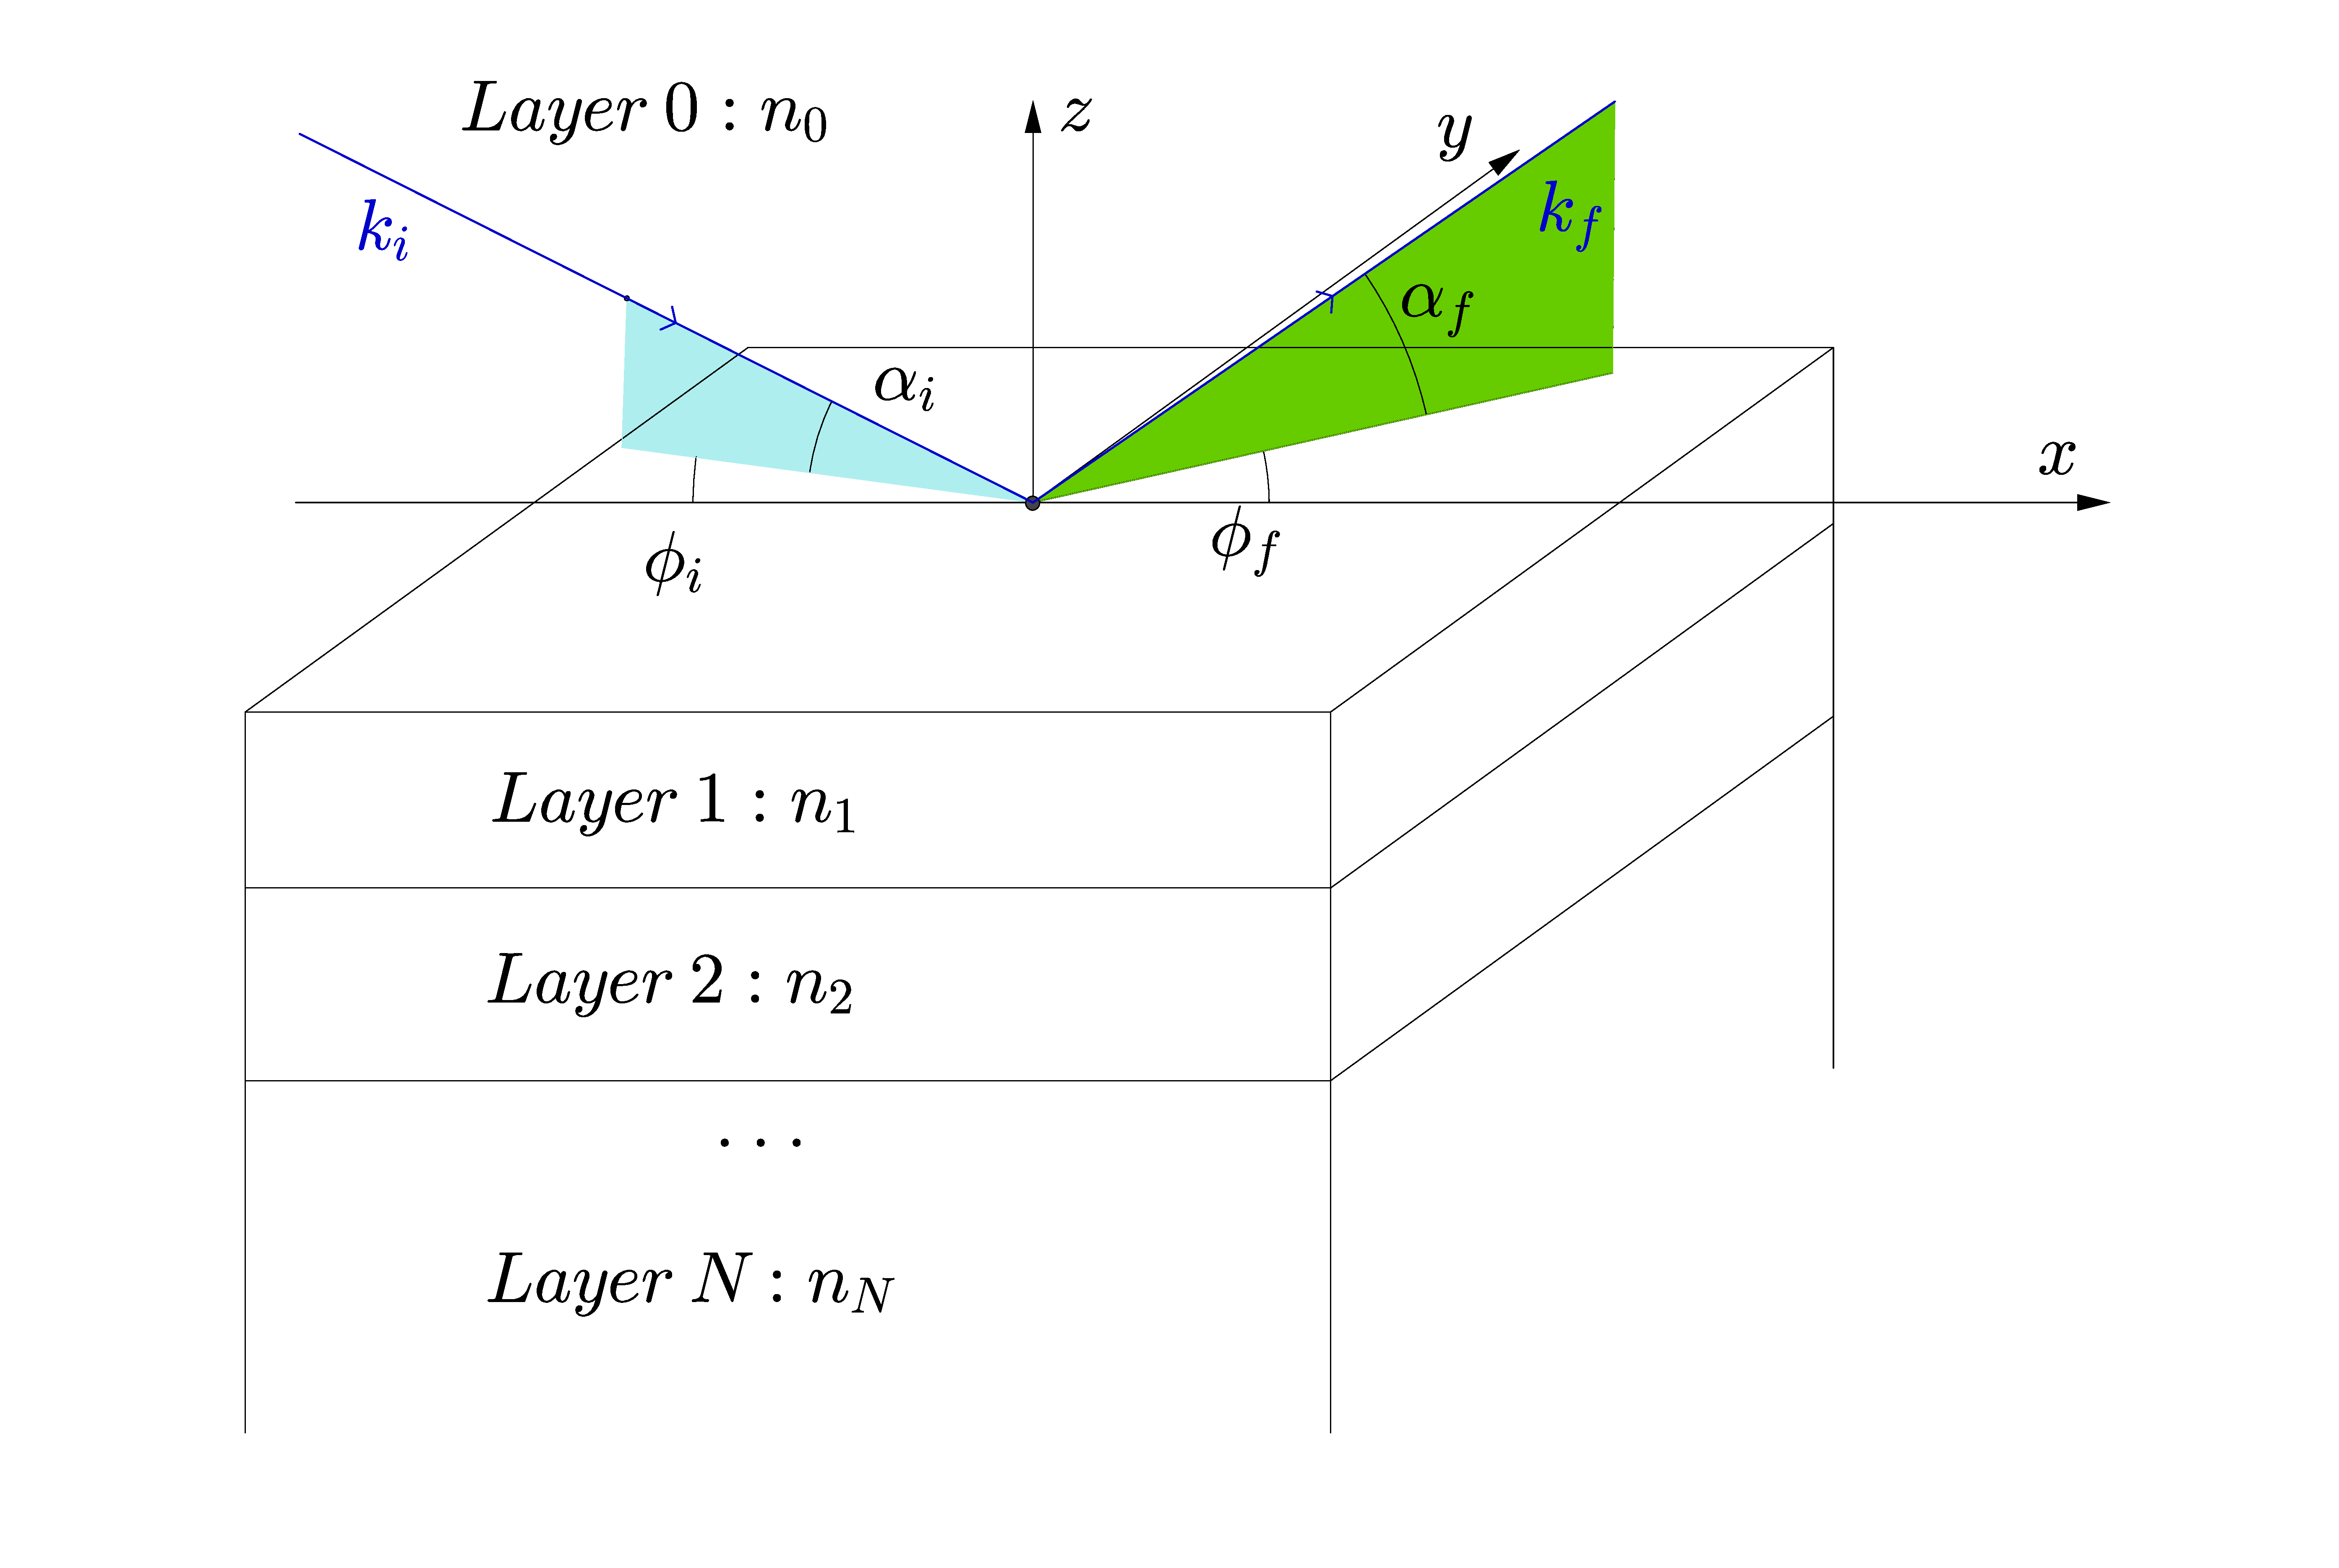
\includegraphics[clip=, width=120mm]{Figures/multilayer3d3.eps}
  \caption[Representation of the scattering geometry.]{Representation of the scattering geometry. $n_j$ is
    the refractive index of layer $j$ and $\alpha_i$ and $\phi_i$ are the incident
    angle of the wave propagating. $\alpha_f$ is the exit angle with respect to the sample's surface and
$\phi_f$ is the scattering angle with respect to the scattering
plane. }
  \label{fig:multil3d}
\end{figure}

\noindent The input beam is assumed to be monochromatic without any
spatial divergence.\\ %\textbf{polarization term?}

\subsection{Units}
By default the angles are expressed in radians and the lengths are given in
nanometers.  But it is possible to use other units by
specifying them right after the value of the corresponding
parameter like, for example, \Code{20.0*micrometer}.


\subsection{Programs}

The examples presented in the next paragraphs are written in Python. For tutorials about this
   programming language, the users are referred to \cite{Pythonref}.

%\noindent Note about the version of C++ and Python to run the examples.\\
%\noindent Where can the following examples be found?\\
%\noindent What is the command to run the examples?

%%%%%%%%%%%%%%%%%%%%%%%%%%%%%%%%%%%%%%%%%%%%
\mysection{Example 1}{Example 1: Two types of islands on top of
  substrate. No interference function} \SecLabel{Example1Python}
% \sectionmark{Example 1}

In this example, we simulate the scattering from a mixture of
cylindrical and prismatic nanoparticles without any interference
between them. These particles are placed in air, on top
of a substrate.\\ We are going to go through each step of the
simulation. The Python script specific to each stage will be given at
the beginning of the description. But for the sake of completeness the full code is given
at the end of this section (Listing~\ref{script_ex1}). \\

\noindent We start by importing different functions from external
modules (line~\ref{import_lib}), for example NumPy, which
is a fundamental package for scientific computing with Python \cite{NumPyURL}.  In particular, line~\ref{import_end}
imports the features of \BornAgain\ software.\\

\begin{lstlisting}[language=python, style=eclipseboxed,name=ex1,nolol]
import sys, os, numpy @\label{import_lib}@

from libBornAgainCore import * @\label{import_end}@
\end{lstlisting}


 %%%%%%%%%%%%%  
\myparagraph{\underline{First step:} Defining materials} 
 

\begin{lstlisting}[language=python, style=eclipseboxed,name=ex1,nolol]
def RunSimulation(): @\label{def_function}@
    #  defining materials @\label{material1}@
    mAmbience = MaterialManager.getHomogeneousMaterial("Air", 0.0, 0.0)  @\label{material2}@
    mSubstrate = MaterialManager.getHomogeneousMaterial("Substrate",
    6e-6, 2e-8) @\label{material3}@
    mParticle = MaterialManager.getHomogeneousMaterial("Particle", 6e-4,
  2e-8 ) @\label{materialparticle}@
\end{lstlisting}

\noindent Line~\ref{def_function} marks the beginning of the
function to define and run the simulation. 

\noindent Lines~\ref{material2}, \ref{material3} and \ref{materialparticle} define different
materials using function \Code{getHomogeneousMaterial} from class
\Code{MaterialManager}. The general syntax is the following 

\begin{lstlisting}[language=python, style=eclipse,numbers=none]
<material_name> = MaterialManager.getHomogeneousMaterial("name", delta, beta)
\end{lstlisting}

\noindent where \Code{name} is the name of the
material associated with its complex refractive index
n=1-\Code{delta} +i \Code{beta}. \Code{<material\_name>} is later used when
referring to this particular material. The three defined materials in this example are \Code{Air} with a refractive
index of 1 (\Code{delta = beta =0}), a \Code{Substrate} associated with a complex refractive index
equal to $1-6\times 10^{-6} +i2\times 10^{-8} $, and the material of particles, whose refractive index is \Code{n}$=1-6\times 10^{-4}+i2\times 10^{-8}$.\\\\

%\noindent \underline{Remark:} there is no condition on the choice of \Code{name}. 
 %%%%%%%%%%%%% 
\myparagraph{\underline{Second step:} Defining the particles} 

\begin{lstlisting}[language=python,style=eclipseboxed,name=ex1,nolol]
    # collection of particles @\label{particles1}@
    cylinder_ff = FormFactorCylinder(5*nanometer, 5*nanometer) @\label{particlescyl1}@
    cylinder = Particle(mParticle, cylinder_ff) @\label{particlescyl2}@
    prism_ff = FormFactorPrism3(5*nanometer, 5*nanometer) @\label{particlesprism1}@
    prism = Particle(mParticle, prism_ff) @\label{particlesprism2}@
\end{lstlisting}

 \noindent We implement two different shapes of particles: cylinders and
 prisms (\textit{i.e.} elongated particles with a constant equilateral triangular cross section).\\ All particles implemented in \BornAgain\ are defined by their
 form factors, their sizes and the material
  they are made of. Here, for the
  cylindrical particle, we input its radius and height.  For the prism, 
  the possible inputs are the length of one side of its equilateral triangular
  base and its height.\\

%\noindent In line~\ref{complx_ref_index}, we define the complex refractive index
%associated with both particle shapes: \Code{n}$=1-6\times 10^{-4}+i2\times 10^{-8}$.\\
  
\noindent In order to define a particle, we proceed in two steps. For example for
the cylindrical particle, we first specify the form factor of a cylinder with 
its radius and height, both equal to 5 nanometers in this particular
case (see line~\ref{particlescyl1}). Then we associate this shape with
the constituting material as in line~\ref{particlescyl2}.\\

\noindent The same procedure has been applied for the prism in lines~\ref{particlesprism1} and \ref{particlesprism2} respectively.
 %%%%%%%%%%%%% 
\myparagraph{\underline{Third step:} Characterizing the layers and assembling the sample} 

\noindent \textbf{Particle decoration} \\
  

\begin{lstlisting}[language=python, style=eclipseboxed, name=ex1,nolol]
    particle_decoration = ParticleDecoration()  @\label{particlesdecor1}@
    particle_decoration.addParticle(cylinder, 0.0, 0.5)  @\label{particlesdecor2}@
    particle_decoration.addParticle(prism, 0.0, 0.5)@\label{particlesdecor3}@
    interference = InterferenceFunctionNone()  @\label{particlesnointerf}@
    particle_decoration.addInterferenceFunction(interference)  @\label{particlesinterf}@
\end{lstlisting}

\noindent The object which holds the information about the positions and densities of particles
in our sample is called \Code{ParticleDecoration}
(line~\ref{particlesdecor1}). We use the associated function \Code{addParticle}
for each particle shape (lines~\ref{particlesdecor2}, \ref{particlesdecor3}). Its general
syntax is 

\begin{lstlisting}[language=python, style=eclipse,numbers=none]
addParticle(<particle_name>, depth, abundance) 
\end{lstlisting}

\noindent  where \Code{<particle\_name>} is the name used to define the particles
(lines~\ref{particlescyl2} and \ref{particlesprism2}), \Code{depth}
(default value =0)
is the vertical position, expressed in nanometers, of the particles in a given layer (the
association with a particular layer will be done during the next step) and
\Code{abundance} is the proportion of this type of particles, 
normalized to the total number of particles. Here we have 50\% of cylinders
and 50\% of prisms. \\ 

\ImportantPoint{Remark:}{Depth of particles\\
The vertical positions of particles in a layer are given in relative
coordinates. For the top layer, the bottom corresponds to
\Code{depth}=0 and negative values would correspond to particles
floating above layer 1 since the vertical axis, shown in \reffig{multil3d} is pointing upwards. But for all the other layers, it is the top of the
layer which corresponds to \Code{depth}=0.}\\


\noindent Finally lines~\ref{particlesnointerf} and
\ref{particlesinterf} specify that there is \textbf{no coherent interference} between
the waves scattered by these particles. The intensity is calculated by
the incoherent sum of the scattered waves: $\langle |F_n|^2\rangle$,
where $F_n$ is the form factor associated with the particle of type $n$.  The way these waves
interfere imposes the horizontal distribution of
the particles as
the interference reflects the long or short-range order of the
particles distribution (\textbf{see Theory}). On the contrary, the vertical position is
imposed when we add the particles in a given layer by parameter \Code{depth}, as shown in lines~\ref{particlesdecor2} and \ref{particlesdecor3}. \\

\noindent \textbf{Multilayer}\\
  
\begin{lstlisting}[language=python, style=eclipseboxed,name=ex1,nolol]
    # air layer with particles and substrate form multi layer  @\label{sampleassembling}@
    air_layer = Layer(mAmbience)  @\label{airlayer}@
    air_layer.setDecoration(particle_decoration)  @\label{airlayerdecorator}@
    substrate_layer = Layer(mSubstrate, 0)  @\label{substratelayer}@
    multi_layer = MultiLayer()  @\label{multilayercanvas}@
    multi_layer.addLayer(air_layer)  @\label{layerairdecor}@
    multi_layer.addLayer(substrate_layer)  @\label{layersubstrate}@
\end{lstlisting}

\noindent We now have to configure our sample. For this first example,
the particles, \textit{i.e.} cylinders and prisms, are on top of a substrate in an
air layer. \textbf{The order in which we define these layers is important: we
start from the top layer down to the bottom one}.\\

\noindent Let us start with the air layer. It contains the particles. In
line~\ref{airlayer}, we use the previously defined \Code{mAmbience}
(="air" material) (line~\ref{material2}). The command written in line~\ref{airlayerdecorator} shows that this layer is decorated by adding the
particles using the function \Code{particle\_decoration} defined in
lines~\ref{particlesdecor1}-\ref{particlesinterf}. The substrate layer
only contains the substrate material (line~\ref{substratelayer}).\\%Note that the
%\Code{depth} is referenced to the bottom of the top layer (negative
%values would correspond to particles floating above layer 1 as
%the vertical axis is pointing upwards). 
 
\noindent There are different possible syntaxes to define a layer. As shown in
lines~\ref{airlayer} and \ref{substratelayer}, we can use
\Code{Layer(<material\_name>,thickness)} or
\Code{Layer(<material\_name>)}. The second case corresponds
to the default value of the \Code{thickness}, equal to 0. The \Code{thickness} is
expressed in  nanometers. \\

\noindent Our two layers are now fully characterized. The sample is assembled using
\Code{MultiLayer()} constructor (line~\ref{multilayercanvas}): we start with the air layer decorated
with the particles (line~\ref{layerairdecor}), which is the layer at
the top and end with the bottom layer, which is the
substrate (line~\ref{layersubstrate}).
 %%%%%%%%%%%%% 
\myparagraph{\underline{Fourth step:} Characterizing the input beam and
output detector and running the simulation} 


\begin{lstlisting}[language=python, style=eclipseboxed,name=ex1,nolol]
    # run simulation  @\label{run1}@
    simulation = Simulation()  @\label{run2}@
    simulation.setDetectorParameters(100,-1.0*degree, 1.0*degree, 
                                100, 0.0*degree, 2.0*degree, True)  @\label{rundetector}@
    simulation.setBeamParameters(1.0*angstrom, 0.2*degree, 0.0*degree)  @\label{runbeam}@
    simulation.setSample(multi_layer)  @\label{runsample}@
    simulation.runSimulation()  @\label{runsimul}@
\end{lstlisting}


\noindent The first stage is to define the \Code{Simulation()} object (line~\ref{run2}). Then we define the detector (line~\ref{rundetector}) and beam
parameters (line~\ref{runbeam}), which are associated with the
sample previously defined (line~\ref{runsample}). Finally we run
the simulation (line~\ref{runsimul}). Those functions are part of the Simulation
class.  The
different incident and exit angles are
shown in \reffig{multil3d}. \\

\noindent The detector parameters are set using ranges of angles via
the function:\\

\noindent \Code{setDetectorParameters(n\_phi, phi\_f\_min,
  phi\_f\_max,\\ \phantom{setDetectorParameters(}n\_alpha, alpha\_f\_min, alpha\_f\_max, isgisaxs\_style=false)}, \\

\noindent where \Code{n\_phi=100} is the number of iterations for $\phi_f$,\\ \Code{phi\_f\_min=-1.0*degree} and \Code{phi\_f\_max=1.0*degree}
are the minimum and maximum values respectively of $\phi_f$, \\ \Code{n\_alpha=100} is
the number of iterations for $\alpha_f$,\\ \Code{alpha\_f\_min=0.0*degree} and \Code{alpha\_f\_max=2.0*degree} 
are the minimum and maximum values respectively of
$\alpha_f$. \\
\Code{isgisaxs\_style=True} (default value = \Code{False}) is a boolean
used to characterise the structure of the output data. If
\Code{isgisaxs\_style=True}, the output data is binned at constant
values of the sine of the output angles, $\alpha_f$ and $\phi_f$, otherwise it is binned
at constant values of these two angles.\\


\noindent For the beam the function to use is
\Code{setBeamParameters(lambda, alpha\_i, phi\_i)}, where\\
\Code{lambda=1.0*angstrom} is the incident beam wavelength,
\Code{alpha\_i=0.2*degree} is the incident
grazing angle on the surface of the sample,
\Code{phi\_i=0.0*degree} is the in-plane
direction of the incident beam (measured with respect to the
$x$-axis).\\ 

\noindent \underline{Remark}: Note that, except for
\Code{isgisaxs\_style}, there are no default values implemented for the
parameters of the beam and detector.\\

\noindent Line~\ref{runsimul} shows the command to run the simulation using the
previously defined setup.
%%%%%%%%%%%%%
\myparagraph{\underline{Fifth step:} Saving the data} 


\begin{lstlisting}[language=python, style=eclipseboxed,name=ex1,nolol]
    # retrieving intensity data
    return GetOutputData(simulation) @\label{outputdata}@
\end{lstlisting}


\noindent In line~\ref{outputdata} we obtain the simulated intensity
as a function of outgoing angles $\alpha_f$ and $\phi_f$ for further
uses (plots, fits,\ldots) as a NumPy array containing
\Code{n\_phi}$\times$\Code{n\_alpha}
datapoints. Some options are provided by \BornAgain. For example, \reffig{output_ex1} shows the two-dimensional
contourplot of the intensity as a function of $\alpha_f$ and
$\phi_f$. 

\begin{figure}[h]
  \begin{center}
   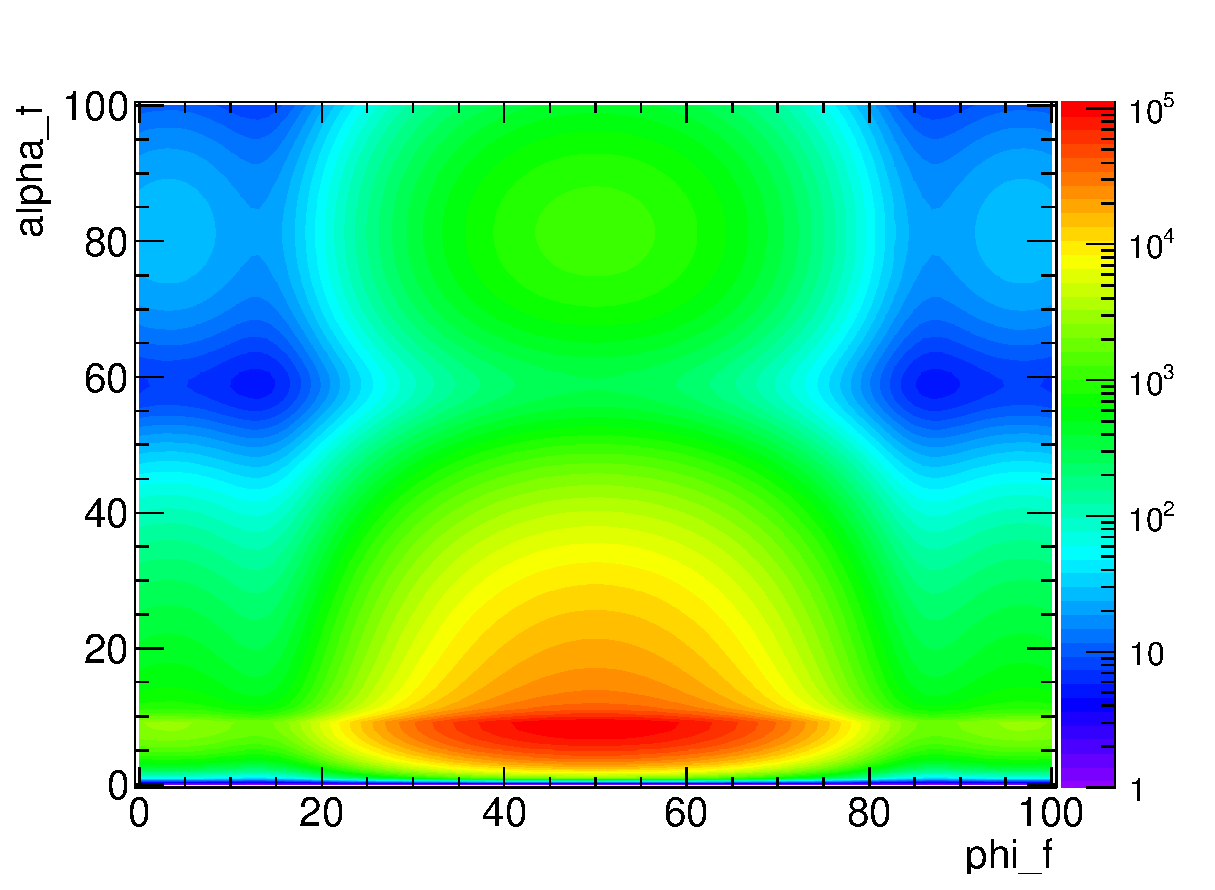
\includegraphics[clip=true, width=120mm]{Figures/Manual_ex1.eps}
  \end{center}
  \caption[Example 1: Simulated grazing-incidence small-angle X-ray scattering from a mixture of
cylindrical and prismatic nanoparticles without any interference, deposited on top
of a substrate]{Figure of example 1: Simulated grazing-incidence small-angle X-ray scattering from a mixture of
cylindrical and prismatic nanoparticles without any interference, deposited on top
of a substrate. The input beam is characterized by a wavelength
$\lambda$ of 1~\AA\ and incident angles $\alpha_i=0.2^{\circ}$, $\phi_i=0^{\circ}$. The
cylinders have a radius and a height both equal to 5~nm, the prisms
are characterized by a side length equal to 5~nm and they are also 5~nm high. The
material of the particles has a refractive index of $1-6\times 10^{-4}+i2\times 10^{-8}$. For the substrate
it is equal to $1-6\times 10^{-6} +i2\times 10^{-8} $. The colorscale
is associated with the output intensity in arbitrary units. }
\label{fig:output_ex1}
\end{figure}

\newpage
\begin{lstlisting}[caption={Python script of example 1},
  label=script_ex1,captionpos=b,escapeinside={@}{@} ,language=python,style=eclipse, numbers= none,frame = leftline ,
      framerule = 2mm ,
      rulecolor = \color{lightgrey},
      breaklines = true]
import sys, os, numpy 

sys.path.append(os.path.abspath(os.path.join(os.path.split(__file__)[0],'..', '..', '..', 'lib')))

from libBornAgainCore import * 

def RunSimulation():
    #  defining materials 
    mAmbience = MaterialManager.getHomogeneousMaterial("Air", 0.0, 0.0 ) 
    mSubstrate = MaterialManager.getHomogeneousMaterial("Substrate",
    6e-6, 2e-8) 
    mParticle = MaterialManager.getHomogeneousMaterial("Particle", 6e-4, 2e-8 )
    # collection of particles 
    cylinder_ff = FormFactorCylinder(5*nanometer, 5*nanometer) 
    cylinder = Particle(mParticle, cylinder_ff) 
    prism_ff = FormFactorPrism3(5*nanometer, 5*nanometer) 
    prism = Particle(mParticle, prism_ff) 
    particle_decoration = ParticleDecoration()  
    particle_decoration.addParticle(cylinder, 0.0, 0.5)  
    particle_decoration.addParticle(prism, 0.0, 0.5)  
    interference = InterferenceFunctionNone()  
    particle_decoration.addInterferenceFunction(interference)  
    # air layer with particles and substrate form multi layer 
    air_layer = Layer(mAmbience)  
    air_layer.setDecoration(particle_decoration)
    substrate_layer = Layer(mSubstrate, 0) 
    multi_layer = MultiLayer()  
    multi_layer.addLayer(air_layer) 
    multi_layer.addLayer(substrate_layer) 

    # build and run simulation  
    simulation = Simulation()  
    simulation.setDetectorParameters(100,-1.0*degree, 1.0*degree, 
                                    100, 0.0*degree, 2.0*degree, True) 
    simulation.setBeamParameters(1.0*angstrom, 0.2*degree, 0.0*degree) 
    simulation.setSample(multi_layer) 
    simulation.runSimulation()  

    # retrieving intensity data
     return GetOutputData(simulation)
\end{lstlisting}

% \newpage
% \subsection{Hello, minted}
% 
% \begin{minted}[linenos=true, frame=single]{python}
% mAmbience = MaterialManager.getHomogeneousMaterial("Air", 1.0, 0.0 )
% mSubstrate = MaterialManager.getHomogeneousMaterial("Substrate", 1.0-6e-6, 2e-8 )
% n_particle = complex(1.0-6e-4, 2e-8)
% cylinder_ff = FormFactorCylinder(5*nanometer, 5*nanometer)
% cylinder = Particle(n_particle, cylinder_ff)
% prism_ff = FormFactorPrism3(5*nanometer, 5*nanometer)
% prism = Particle(n_particle, prism_ff)
% particle_decoration = ParticleDecoration()
% particle_decoration.addParticle(cylinder, 0.0, 0.5)
% particle_decoration.addParticle(prism, 0.0, 0.5)
% interference = InterferenceFunctionNone()
% particle_decoration.addInterferenceFunction(interference)
% # air layer with particles and substrate form multi layer
% air_layer = Layer(mAmbience)
% air_layer_decorator = LayerDecorator(air_layer, particle_decoration)
% substrate_layer = Layer(mSubstrate, 0)
% multi_layer = MultiLayer()
% multi_layer.addLayer(air_layer_decorator)
% multi_layer.addLayer(substrate_layer)
% 
% # build and run experiment
% simulation = Simulation()
% simulation.setDetectorParameters(100,-1.0*degree, 1.0*degree, 100, 0.0*degree, 2.0*degree, True)
% simulation.setBeamParameters(1.0*angstrom, -0.2*degree, 0.0*degree)
% simulation.setSample(multi_layer)
% simulation.runSimulation()
% \end{minted}

\section{Example 2}





%List of notations\\  Bugs\\ License agreement\\ Directory layout \\ FAQ \\ Future development.

%\appendix
%%Appendix
\chapter{Implemented classes}

\begin{itemize}
\item Particle decoration
\item Layer
\item MultiLayer
\item Simulation
\end{itemize}

\chapter{Form factors}
% plots of particles + orientation of the axes
% plots of the form factors

\begin{itemize}
\item Parallelepiped (\texttt{FormFactorParallelepiped})

\begin{equation}
F() = 4H R^2\exp(i q_z H/2) \frac{sin(q_xR)}{q_x R}\frac{ \sin(q_yR)}{q_y R}\frac{\sin(q_z H/2)}{q_z H/2}
\end{equation}
\item Pyramid (\texttt{FormFactorPyramid})

\begin{align*}
        q_1 &=(H/2)((q_x-q_y)/\tan(\alpha) + q_z)\\
        q_2 &=(H/2)((q_x-q_y)/\tan(\alpha) - q_z)\\
        q_3 &=(H/2)((q_x+q_y)/\tan(\alpha) + q_z) \\
        q_4 &=(H/2)((q_x+q_y)/\tan(\alpha) - q_z)\\
        K_1 &= \frac{\sin(q_1)}{q_1} \exp(i q_1)  + i \frac{\sin(q_2)}{q_2} \exp(-i q_2)\\
        K_2 &= -i \frac{sin(q_1)}{q_1} exp(i q_1) +i \frac{\sin(q_2)}{q_2} \exp(-i q_2)\\
        K_3 &= \frac{\sin(q_3)}{q_3}\exp(i q_3)    + \frac{\sin(q_4)}{q_4} \exp(-i q_4)\\
        K_4 &= -i \frac{\sin(q_3)}{q_3} \exp(i q_3) + i \frac{\sin(q_4)}{q_4} \exp(-i q_4)\\     
  F() &= \frac{H}{q_x q_y} [ K_1 \cos( (q_x-q_y)R ) + K_2 \sin( (q_x-q_y)R ) - K_3 \cos( (q_x+q_y) R ) - K_4 \sin( (q_x+q_y) R )]
   \end{align*}
	
\item Cylinder (\texttt{FormFactorCylinder})

  \begin{equation}
 F()=   H  \frac{\sin(q_ z H/2)}{q_z H/2} \exp(i q_ z H/2) 2\pi R^2 \frac{J_1(|q_{\parallel} R |)}{|q_{\parallel} R| }
 \end{equation}
 

\item Prism3 (\texttt{FormFactorPrism3})

\begin{equation}
    F()= 2 \sqrt{3}\frac{\exp(-i q_y R/\sqrt{3})}{q_x^2-3q_y^2}[\exp(i \sqrt{3} q_y R ) -\cos(q_x R)-i \sqrt{3} q_y R \frac{\sin(q_x R)}{q_x R}]   H \frac{\sin(q_z H/2 )}{q_z H/2} \exp(i q_z H/2)
\end{equation}

\item Sphere (\texttt{FormFactorSphere})

\begin{equation}    
return 2\pi \exp(i q_z (H-R))\int_{R-H} ^{R} R_z^2 \frac{J_1(|q_p*R_z|) }{|q_p*R_z|}
        \exp(i q_z*Z)
\end{equation}


\item Full sphere (\texttt{FormFactorFullSphere})

\begin{equation}
radial = 4\pi R^3*\frac{\sin(q R) - q R*\cos(q R)}{(qR)^3}
\end{equation}

\item Box (\texttt{FormFactorBox})

\begin{equation}
F()= 4H R W\exp(i q_z H/2) \frac{\sin(q_x R)}{q_x R} \frac{  \sin(q_y W) }{q_y W}\frac{\sin(q_z H/2)}{q_z H/2}
\end{equation}
    
	
\end{itemize}

\chapter{Interference functions}

\begin{itemize}
\item	No interference 
\item	decoupling approximation 	
\item 	local mono disperse approximation 
\item 	size spacing approximation 
\end{itemize}


\chapter{Pair correlation functions}
\begin{itemize}
\item The Debye hard core 
\item The gaussian
\item The Lennard-Jonnes  	
\item The gate pair correlation 	
\item The Debye hard core with power-law decrease  	
\item The Zhu pair correlation function 	
\item The Venables pair correlation function 	
\item The bidimensional hard core pair function.
\end{itemize}	


%\printindex
%generate an index - hyperref

\bibliography{ref}
\bibliographystyle{unsrt}




\end{document}

